% MUST use a4paper option
% MAY use twoside, smaller font, and other class
\documentclass[a4paper,12pt]{article}
% Use UTF-8 encoding in input files
\usepackage[utf8]{inputenc}
% NOTE: If you are writing in English, un-comment the following line:
% \usepackage[swedish,english]{babel}
% Use the template for thesis reports
\usepackage{UppsalaExjobb}

%legender till bilder
\usepackage{overpic}
\usepackage{pict2e}

% Useful font packages for maths and symbols
\usepackage{amssymb,amsmath,amsthm,amsfonts}
\usepackage{graphicx,wrapfig,lipsum}
% ser till att floats inte hoppar till en annan section
\usepackage{placeins}
%\usepackage{flafter}

\usepackage{enumerate}
\usepackage{tabularx}
\usepackage{subcaption}
\DeclareCaptionLabelFormat{cont}{#1~#2\alph{ContinuedFloat}}
\captionsetup[ContinuedFloat]{labelformat=cont}

% to get the same vertical spacing as \paragraph
\newcommand{\emptyparagraph}{\paragraph{}\hspace{-1em}}

\definecolor{background}{gray}{0.95}
\definecolor{cadmiumgreen}{rgb}{0.0, 0.42, 0.24}

% for nice code listings
\usepackage{listings}
\lstdefinelanguage{jsx}{
  keywords={const, class, extends, typeof, new, true, false, catch, function, return, null, catch, switch, var, if, in, while, do, else, case, break},
  keywordstyle=\color{blue}\bfseries,
  keywords=[2]{export, boolean, throw, implements, import, this, document, ReactDOM, console},
  keywordstyle=[2]\color{YellowGreen}\bfseries,
  keywords=[3]{<div>, </div>, <p>, </p>, />},
  keywordstyle=[3]\color{Plum},
  alsoletter={<>/},
  identifierstyle=\color{black},
  sensitive=false,
  comment=[l]{//},
  morecomment=[s]{/*}{*/},
  commentstyle=\color{purple}\ttfamily,
  stringstyle=\color{red}\ttfamily,
  morestring=[b]',
  morestring=[b]"
}

\lstset{
   backgroundcolor=\color{background},
   %extendedchars=true,
   basicstyle=\footnotesize\ttfamily,
   numbers=left,
   numberstyle=\footnotesize,
   captionpos=b,
   escapechar=|
}

% Reference name
%\usepackage{nameref}

\usepackage{tikz}
\usetikzlibrary{arrows,shapes,decorations.pathmorphing,calc,positioning}
\tikzset{
  >=stealth'
}

% bara för att få den kortare
\newcommand{\li}{\lstinline}

% visar vart overfulla saker ligger
%\overfullrule=20pt

% fixa en konstig varning från fancyhdr som kom från ingenstans
\setlength{\headheight}{14.7pt}

% Designval: per default används styckesindrag, men ibland blir det snyggare/mer lättläst med tomrad mellan stycken. Det åstadkoms av de följande raderna.
% Tycker ni om styckesindrag mera, kommentera bort nästa två rader.
\parskip=0.8em
\parindent=0mm

% Designval: vill ni ha en box runt figurer istället för strecken som är default, av-kommentera raden nedan. Obs att både \floatstyle och \restylefloat behövs.
%\floatstyle{boxed} \restylefloat{figure}

\begin{document}
% För att ställa in parametrar till IEEEtranS/IEEEtranSA behöver detta ligga här (före första \cite).
% Se se IEEEtran/bibtex/IEEEtran_bst_HOWTO.pdf, avsnitt VII, eller sista biten av IEEEtran/bibtex/IEEEexample.bib.
\bstctlcite{rapport:BSTcontrol}


% Set title, and subtitle if you have one
%\title{Ett verktyg för att bygga avtal och en chattbott för att ge enkel rådgivning} % och uppsatsmetodik
\title{Tjänst för skapande och ifyllande av juridiska avtal i ett interaktivt dialogsystem}
% Use this if you have a subtitle
%\subtitle{Botten som är toppen!}
% Set author names, separated by "\\ " (don't forget the space)
% List authors alphabetically by last name (unless someone did significantly more/less)
\author{Johan Boström \\ Daniel Jansson \\ Martin Larsson \\ Erik Rimskog}
% Set the date and year - use the right language!
\date{\begin{otherlanguage}{swedish}  %\foreignlanguage doesn't seem to affect \today?
\today
\end{otherlanguage}}

% Only need to set the year if it differs from the current year
%\year=2018

% Ange handledare, ämnesgranskare, examinator om dessa finns
% Extern handledare: t.ex på företag ni arbetat med?
\exthandledare{Jimmy Eriksson, Sisyfos AB}
% Intern handledare
\handledare{Björn Victor och Mats Daniels}
% Ämnesgranskare används inte på Självständigt arbete i IT
%\reviewer{NN}
% På Självständigt arbete i IT är detta BV
\examinator{Björn Victor}

% Programnamn på svenska och engelska
\progname{Civilingenj{\"o}rsprogrammet i informationsteknologi}{Master Programme in Computer and Information Engineering}

% Utgivare
\enhetsnamn{Institutionen för \\ informationsteknologi}
\besoksadress{ITC, Polacksbacken\\ Lägerhyddsvägen 2}
\postadress{Box 337 \\ 751 05 Uppsala}
\hemsida{http:/www.it.uu.se}

% Set the name of the series, and the number in the series
\seriesname{Självständigt arbete i informationsteknologi}
% \seriesname{Uppsatsmetodik}

% OBS: Gäller bara exjobb i årskurs 5
% Get a series number, e.g. from Studentservice Ångström
%\seriesnumber{UPTEC IT16~0xx}
% Use the appropriate ISSN for the series
%\issn{ISSN 1401-5749}
% Usually this is where it is printed
%\printer{Ångströmlaboratoriet, Uppsala universitet}

% This creates the title page
\maketitle

% Change to frontmatter style (e.g. roman page numbers)
\frontmatter

\begin{abstract}
%Abstract, always in English, about 10-20 lines. Do not use references; do not use formulas if they can be avoided.
%\begin{enumerate}
%\item What is the problem/issue/subject?
%\item How was the problem solved/attacked?
%\item What are the results, how well was the problem solved?
%\item How good are the results, how useful are they?
%\end{enumerate}
%The abstract should be understandable without reading the whole report (and the rest of the report should be understandable without reading the abstract). You can reuse text/phrases from the Introduction.

Everyone will, sooner or later, have to sign a legally binding agreement. Two examples of such agreements are purchase agreements for a car and a consultant agreement for when someone is recruited as a consultant. Many of these agreements follow a standard template and rarely change. \\

It is perceived as cumbersome and costly for individuals to contact a lawyer for the assistance of standardised agreements and that legal terminology can be perceived as alien and frightening. Our thesis is that the handling of these standardised agreements can be streamlined and thus improve the work flow of a legal firm.\\

Our solution to this problem is a system that allows for a costumer to communicate with a chatbot. This chatbot can identify and fill in the agreement that is best suited for the users situation. The agreements available to the system are created by a lawyer through an administrative tool. Using this tool the lawyer can create new templates for agreements and also review the agreements that has been filled in by users.

The project resulted in a chat interface for the user and an administrative tool in which an administrator can create and manage templates for contracts. Based on short messages from the user, the system is capable of choosing a contract among those created in administrative tool and recommend it to the user.

\end{abstract}

\begin{sammanfattning}
%Sammanfattning, alltid på svenska. Se till att det står samma saker i det svenska och det engelska abstractet.
%\begin{enumerate}
%\item Vad är problemet, ämnet?
En privatperson kommer förr eller senare behöva teckna ett juridisk bindande avtal. Två exempel på sådana avtal är köpeavtal för en bil eller ett konsultavtal när någon anställts som konsult. Många av dessa avtal följer en standardiserad mall och ändras sällan. Det upplevs som omständligt och kostsamt för privatpersoner att kontakta en jurist för assistans med standardiserade avtal samt att juridisk terminologi kan upplevas som främmande och skrämmande. Vår tes är att hanteringen av dessa standardiserade avtal kan effektiviseras och därmed förbättra en juristfirmas arbetsflöde.

Vår lösning på problemet är ett system som ger en kund möjlighet att föra en dialog med en chattbott som identifierar och hjälper kunden att fylla i det avtal den behöver.
De avtal som finns tillgängliga har en jurist tidigare har skapat med hjälp av vår administratörssida. På denna sida kan juristen skapa nya avtalsmallar samt se tidigare ifyllda avtal.

Projektet resulterade i ett chattgränssnitt för användaren och ett administratörsverktyg där en administratör kan skapa och hantera avtalsmallar. Systemet är kapabelt att rekommendera avtal baserat på korta meddelanden från användaren. De avtal som kan rekommenderas är de som skapats i administratörsverktyget.

%mats andra kommentar


%\end{enumerate}

%Ca 10-20 rader. Använd inte referenser; ej heller formler om det går att undvika.
\end{sammanfattning}

% Innehållsförteckningen här.
\tableofcontents

% Här kan man också ha \listoffigures, \listoftables

\cleardoublepage


% Change to main matter style (arabic page numbers, reset page numbers)
\mainmatter

% Here comes the text of the report.

%\section*{Hur ni använder detta malldokument}
%Titta i källdokumentet för diverse inställningar för författare, titel, etc.
%
%\emph{OBSERVERA} att de ``fasta fält'' som blir på svenska (trots att ni ställt in engelska med \texttt{babel}), som Examinator, Handledare, datum på framsidan osv, \emph{ska} vara på svenska oavsett språk i rapporten. Abstract ska alltid vara på engelska, medan Sammanfattning alltid ska vara på svenska.
%
%I flera appendix finns mer info som inte gäller rapportstrukturen.
%
%I era inlämningar, ta bort (eller kommentera bort) malltexten (beskrivningen av vad som ska stå), men behåll gärna tomma huvudrubriker. Ta också bort mall-appendix.
%
%\subsection*{Generellt}
%Varje numrerat avsnitt ska finnas med i er slutrapport, om inget annat anges.  
%Välj rubrik på svenska eller engelska beroende på ert valda rapportspråk.
%
%Glöm inte att läsa kurslitteraturen~\cite{dawson:projects-in-computing,dawson:projects-in-computing-old}.
%
%% \subsection*{Uppdateringar av detta dokument}
%% \begin{description}
%% \item[2016-05-16]\mbox{}\\
%
%% \end{description}
%
%
%\section*{Att göra}
%En sektion som beskriver läget för rapporten kan vara användbart i ``veckans inlämning'' för att underlätta feedbacken.

\newpage %%%%%%%%%%%%%%%% OBS! Ta bort allt mellan \mainmatter och här (inkl \newpage) i slutversionen (men inte \mainmatter)

\section{Introduktion}
%Beskriv åtminstone samma saker som i abstract, men mer utförligt -- typiskt 1-2 sidor. Spara tekniska detaljer till senare, eftersom läsaren inte är insatt än.

%\begin{enumerate}
%\item Vilket är området ni arbetar inom? Vad är problemet, ämnet?

I Sverige lever åtta av tio sambos utan samboavtal, vilket kan leda till dispyter vid separation, enligt en studie av Verahill~\cite{web:verahill}. Exempelvis, om två ogifta sambos har gemensamma barn och den ena i samboskapet går bort kan den andra tvingas lösa ut sina barns andelar från bostaden, då ogift sambo inte kan ärva av den andre utan avtal~\cite{web:inter-sambo}. Vidare uppger Verahill att det totalt i Sverige står 1~042 miljarder kronor på spel vid separationer (sammanlagt för alla samboskap utan avtal). Som anledning till varför samboavtal inte tecknas anger många att de har en okunskap kring ämnet eller att det upplevs som invecklat. Alltså är okunskap och en benägenhet att spara energi anledningar till att många inte tecknar vissa avtal, trots att det skulle ge individen rättsligt skydd. 

%\item Varför är problemet viktigt/intressant att lösa?
Detta projekt ämnade att utveckla ett system som agerar som en medlare mellan den som söker hjälp och den som erbjuder det. I många fall har kunden en viss uppfattning om vad den vill uppnå och vad dess behov är och vänder sig till en jurist för rådgivning. Men detta är för juristen mycket tidskrävande och begränsar hur många juristen kan ge råd till. Istället kan juristen använda detta system för att skapa mallar för de avtal som de kan tillhandahålla och sedan kan ett stort antal kunder få hjälp av systemet att fylla i dessa.

%\item Hur angreps/löstes problemet? 
%\item Vad är resultaten, hur väl löstes problemet?
%\item Hur bra blev resultaten, hur användbara är de?
Vår lösning för att möjliggöra för jurister att kunna erbjuda mer hjälp bestod av flera delar. Den första delen var ett chattgränssnitt på en webbsida där en användare kan skriva och ställa frågor på svenska. Meddelanden skickas sedan till en server i systemet som använder utomstående verktyg för att tolka meddelandet och avgöra vilken avsikt användaren hade med det för att sedan kunna välja ett passande avtal. Om användaren exempelvis nämner ''varit anställd'' och ''konsult'' kan servern avgöra att ett konsultavtal passar avsikten. Sedan kommer frågor ställas för att få in den information som krävs för att fylla i avtalet. Systemet är kapabelt att tolka användarens avsikter mycket väl, och kan med bara en kort mening som indata avgöra vilket avtal som passar användaren bäst. 

Vilka avtal som kan väljas bestäms av den sista delen av systemet, administratör\-sverktyget. Denna innefattar ett grafiskt verktyg där en administratör skapar avtalsmallar. Här anges vilka avsikter som passar vilka avtal, som att konsultavtal passar när användaren anger ``varit anställd'' och ``konsult''. Administratören kan även lägga till de frågor som behöver ställas för att få den information som krävs för att fylla i avtalet. 

Den datarepresentation som användes för avtalsmallar var tvungen att passa för två ändamål. Den skulle användas för att representera mallar för administratören, samt till analysen av användarens avsikter och behov. Resultatet blev att den passade båda ändamålen.

%\end{enumerate}

%Tänk på att börja introduktionen med en mening eller ännu hellre ett helt stycke som ``fångar'' läsaren och motiverar läsaren att fortsätta läsa.  \emph{Vi har valt att göra ett projekt om X} är relevant för er, men kommer inte att vilja få någon att läsa vidare.  Försök åtminstone få med någon slags bakgrund/kontext och (helst) motivation att fortsätta läsa.  Typ \emph{X är ett programspråk som tagit världen med storm.  Vi vill utforska om man kan kombinera X med Y för att göra\ldots}

%Se till att ni \emph{kommer till kritan snabbt} – man vill inte läsa igenom två stycken text innan man får veta vad ni tänker göra i ert projekt.  Börja t.ex. \emph{inte} med att presentera alla idéer ni inte valt – läsaren vill veta vad ni ska göra, inte vad ni inte ska göra.

%Översiktlig beskrivning av systemet och dess features ska vara under systemdesign / systemstruktur, inte i introduktionen.

%Introduktionen bör vara begriplig för t.ex.~en student i årskursen under, och gärna för en ännu bredare läsarkrets.

\section{Bakgrund}

För någon utan juridisk kunskap kan det vara oklart vad för avtal som behövs och hur de bör vara utformade i den givna situationen. Ett exempel kan vara när någon ska flytta ihop med sin partner. För den oinsatta kan det vara svårt att veta hur ett samboavtal ska vara utformat och vad det bör innehålla, eller i vilka fall det är just ett samboavtal som bör tecknas. Vidare kan bristen av insikt i juridisk terminologi försvåra processen ytterligare.

\subsection{Effektivisering av arbeten}
Människan har alltid strävat mot att effektivisera sitt arbete. Ett exempel på en väl\-etablerad marknad som har blivit effektiviserad är jordbruket. År 1850 var 60\% av USA:s arbetsförda befolkning aktiva inom jordbrukssektorn~\cite{web:job-lost-job-gained}. 120 år senare, år 1970 var det mindre än 5\% aktiva inom jordbrukssektorn. Minskningen var inte en följd av att människan konsumerade mindre livsmedel 120 år senare. Istället hade arbetet inom jordbruk effektiviserats, nya metoder och tillvägagångssätt hade börjat användas. 


Det är inte bara jordbruket som kan effektiviseras, utan även andra arbetsområden. Ett sådant arbetsområde är juridik. Ett exempel inom effektivisering av juridiskt arbete, är en studie som visar att flera delar av en advokats arbete skulle, helt eller delvist, kunna automatiseras ~\cite{web:lawyers-auto}. Mellan 13\% och 23\% av en advokats totala arbete kan automatiseras bort enligt studien. Automatiserbarheten i en arbetsuppgift avgjordes genom att undersöka mängden struktur och repetition i arbetsuppgiften, samt hur förutsägbara och hanterbara olika händelser kopplat till den arbetsuppgiften är. Desto mer struktur i en arbetsuppgift, desto mer automatiserbar ansågs den.

När ett avtal ska tecknas är det mycket repetitivt arbete som behöver göras av den som erbjuder juridisk rådgivning. Det kan vara sådant som att hjälpa någon att fylla i ett avtal, ta fram vilka avtal som kan vara nödvändiga att teckna i den givna situationen eller att tolka juridiska termer. Dessa repetitiva arbeten kan automatiseras och därmed effektivisera juristers arbete. 

\subsection{Chattbottar}
En chattbott är ett system som simulerar mänsklig kommunikation mellan människa och maskin via tal eller skrift~\cite{web:mauldin-chatbot}. 
En av de första vetenskapligt erkända chattbottarna är ELIZA som uppfanns 1966 av Joseph Weizenbaum~\cite{web:dylanavalverde-chatbots}.
ELIZA använder sig av språkteknologi (eng. natural language processing), när ELIZA skapades var begreppet inte etablerat och kallades för natural language conversation (Mer om detta under rubrik~\ref{sec:sprakteknologi})~\cite{web:Eliza-weizenbaum}.
De förekommer fem stycken huvudregler som ELIZA använder sig av~\cite{web:Eliza-weizenbaum}, några av dessa lever kvar än idag. Kärn\-koncept hos dessa regler är att identifiera nyckelord, avsikter och förprogrammerade svar~\cite{web:dylanavalverde-chatbots}.


\begin{figure}[H]
    \centering
    \smallskip
    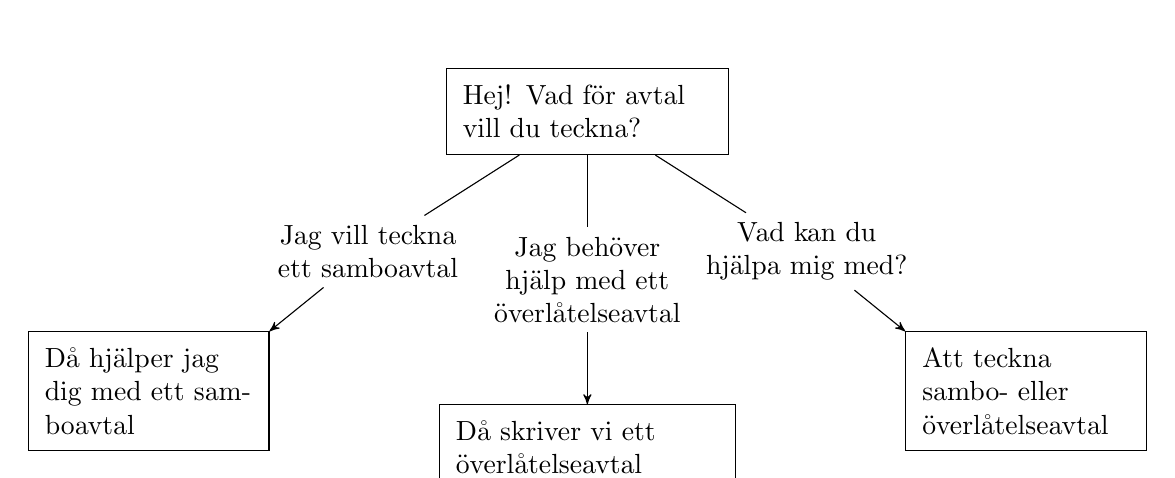
\begin{tikzpicture}[
        rekt/.style={rectangle,draw,inner sep=6pt,align=left,text width=75pt},
        quest/.style={text width=75pt,align=center},
        node distance=90pt
      ]
      \node (TOP) at (0,0) [rekt,text width=90pt] {Hej! Vad för avtal vill du teckna?};
      \node (BIL) [rekt,below left=of TOP] {Då hjälper jag dig med ett samboavtal};
      \node (BIL2) [rekt,below=of TOP, text width=95pt] {Då skriver vi ett överlåtelseavtal};
      \node (BYE) [rekt,below right=of TOP] {Att teckna sambo- eller överlåtelseavtal};
      \node (BILQ) at ($(TOP)!0.5!(BIL)$) [quest] {Jag vill teckna ett samboavtal};
      \node (BIL2Q) at ($(TOP)!0.5!(BIL2)$) [quest] {Jag behöver hjälp med ett överlåtelseavtal};
      \node (BYEQ) at ($(TOP)!0.5!(BYE)$) [quest] {Vad kan du hjälpa mig med?};
      \draw[->] (TOP) -- (BILQ) -- (BIL.north east);
      \draw[->] (TOP) -- (BIL2Q) -- (BIL2);
      \draw[->] (TOP) -- (BYEQ) -- (BYE.north west);
    \end{tikzpicture}
    \smallskip
    \caption{Exempel av dialogträd. Kvadraterna motsvarar meddelande från systemet och meddelande i mitten på dialogpilarna motsvarar svarsalternativ.}
    \label{fig:chattbottar:dialogtree}
\end{figure}
Chattbottar kan använda sig av dialogträd. Dialogträd används för att sätta ramar och regler på hur en användare styrs genom en konversation.
I figur~\ref{fig:chattbottar:dialogtree} ges ett exempel på hur ett dialogträd skulle kunna vara utformat. I det här trädet är både svarsalternativ och svar fördefinierade, det går alltså inte att skriva in svar själv. 
Det här är en föråldrad och begränsad version av ett dialogträd. 
%Dialogträdets styrka och användningsområde är att konversationer tillåts styras och begränsas.


Chattbottar är uppbyggda enligt två olika metoder: AI-baserade och regelbaserade. En AI-baserad chattbott identifierar språk, kontext, avsikt och därefter reagerar med ett svar. En regelbaserad chattbott agerar utifrån en serie av fördefinierade regler~\cite{web:chatbotmagazine-nilima-shah}. En regelbaserad chattbott är uppbyggd på ett regelsystem av villkorssatser där den traverserar framåt i ett dialogträd om ett förbestämt svarsalternativ uppfylls~\cite{web:medium-kumar-shridhar}. Exempel på detta är chattbotten Anna och programmeringspråket Artificial Intelligence Markup Language (AIML)~\cite{web:AIML-anna, web:medium-kumar-shridhar}. 

\subsection{Språkteknologi}
\label{sec:sprakteknologi}
Språkteknologi är ett samlingsnamn för det tvärvetenskapliga forskningsområdet mellan språk- och datavetenskap. Syftet med språkteknologi är att förenkla kommunikation mellan en dator och en människa. Ett exempel på användningsområden är automatiskt översättning mellan olika språk. Språkteknologi är det svenska samlingsnamnet för vad som i engelskan heter Natural Language Processing (NLP) och kommer refereras till som NLP i resterande delar av rapporten~\cite{web:sprakteknologi}.

NLP anses vara en komponent inom  paraplybegreppet artificiell intelligens~\cite{web:5AI}. Som Cambria och White  beskriver uppnår ett NLP-system oftast en form av artificiell intelligens genom maskininlärning~\cite{web:NLPcurves}, där till exempel statistisk NLP har varit en populär metod. En viktig faktor att belysa är att många NLP system ger ett sken av faktiskt intelligent beteende, medan maskiner inte förstår vad de gör. I en analysprocess av naturligt språk i text upplevs uppgiften snarare som en matchning mellan ord och mönster. 
%Här beskriver ni bakgrunden till ert projekt, d.v.s., det som leder fram till er problemformulering.  Vilket är området, omgivningen, kontextet, bakgrunden för projektet (mer detaljerat och djupare än i introduktionen)?  Beskriv området (t.ex. ljudbehandling, studieplaner, visualisering, autism...).  Beskriv uppdragsgivare, om ni har (men inte för detaljerat).  Tänk på att bakgrunden och problemet måste vara på en generell akademisk nivå och inte bara relaterat till en uppdragsgivare.

%Tänk på att bakgrunden kan se längre tillbaka -- hur löste man problemet förr? Innan man började datorisera? Ibland är det både viktigt och intressant (men ibland inte).

%Efter att ha läst bakgrunden ska det vara lätt att förstå syfte/mål och att de är viktiga. Ett typiskt bakgrundsavsnitt är 2-3 sidor.

\section{Problemformulering}\label{sec:syfte}
%Här beskriver ni i princip er problemformulering.  I detta avsnitt ska framgå syfte, mål, och motivation med projektet. 
%Dessa behöver dock \emph{inte} vara separata underrubriker.
Här beskrivs projektets problemformulering, vad vi vill uppnå, vad vi vill åstadkomma och varför vi utför projektet. Dessa beskrivs som syfte, mål och motivation. Vi beskriver även vad vi inte hanterat i projektet under avgränsningar.

De globala hållbarhetsmålen togs i beaktande under projektet. Det är en agenda som antagits av FN:s utvecklingsprogram (UNDP) för att bekämpa problem som fattigdom, minska orättvisor och lösa klimatkrisen. De är uppdelade i 17 kategorier, där varje kategori har ett antal delmål~\cite{web:globalamalen}.

\subsection{Syfte} %\textit{Vart strävar projektet? vad är det övergripande målet, nyttan, effekterna av projektet?  (t.ex. bättre koll på kosthållning, enklare planering av studier\ldots)}

Projektet har två syften, att förenkla för jurister att tillhandahålla avtal för kunder samt att förenkla för kunden att fylla i dessa avtal. Projektet ska resultera i ett system som ger tillgång till juridisk rådgivning till många fler än vad som är möjligt idag. Personer som har låg utbildningsnivå eller som är underpriviligerade på andra sätt får det enklare att förskaffa sig kunskap om vad de kan få för rättsligt skydd och vilka rättigheter de har. 

Systemet kräver inte några juridiska förkunskaper utan all kommunikation sker i tal\-språk (på svenska) för att göra det tydligare och enklare för användaren att förstå. Användaren kan få svar och mer kunskap genom att beskriva sin situation på ett mer vardagligt språk.

Projektet bidrar då till följande globala hållbarhetsmål:
16.3~(Säkerställ tillgång till rättvisa) och
16.10~(Säkerställa allmän tillgång till information och skydda de grund\-läggande friheterna)~\cite{web:globalamalen-16}. Målet 16.3 bidrags till genom att de avtal och den rådgivning som vårt system erbjuder gör att fler får tillgång till avtal som kan skydda dem och därigenom erbjuda rättvisa. Genom att systemet hjälper användare, som inte nöd\-vän\-digt\-vis använder korrekta juridiska termer, att få information och fylla i avtal bidrar systemet även till målet 16.10.

\subsection{Mål} %\emph{Vad ska konkret levereras/utföras av projektet, för att ta oss närmare syftet?}

% - Rådgivning genom chattbott
% - Fylla i avtal om det är ändamålsenligt
% - Se det ifyllda avtalet

Det första målet med projektet är att leverera ett chattgränssnitt i en webbläsare där en kund kan få juridisk rådgivning. När systemet tar emot ett meddelande svarar det med ett rekommenderat avtal att fylla i utifrån det användaren skrivit. Systemet hjälper kunden fylla i avtalet genom att ställa frågor relaterade till avtalet och sparar sedan svaren.

Det andra målet med projektet är att skapa en webbapplikation där administratörer kan skapa avtalsmallar. Dessa mallar utgör de avtal som systemet kan erbjuda kunderna att fylla i. Webbapplikationen kommer också visa alla ifyllda avtal från kunderna.

%Målet med projektet är att leverera ett system som möjliggör för en kund att få juridisk rådgivning genom att skriva med en chattbott i ett egengjort webbläsare. Denna chattbott ska kunna 
%Avgör systemet att det är lämpligt för kunden att fylla i ett specifikt avtal ska frågor ställas för att få den information som krävs för det avtalet. Alltså ska systemet inte kräva att kunden på förhand vet vilket avtal den vill fylla i, utan det ska avgöras utifrån det kunden skriver.


% Efter att konversationen är slut ska kunden även få se det ifyllda avtalet. %Som utgångspunkt kommer gruppen utgå från ett samboavtal som exempel för att lägga grunden för att ett godtyckligt avtal ska kunna fyllas i.

\subsection{Motivation}  %\emph{Varför är projektet viktigt?  Vilka är det viktigt för, vilka externa intressenter finns?  Hur stort är problemet, vad är följden av att det inte är löst, hur bra vore det att lösa?  Vilken ``lucka'' i området täcker ni? Varför är er lösning bättre/annorlunda än andras?}

% Se till att ni i detta avsnitt övertygar läsaren om att problemet finns, att det inte är löst, och att det är viktigt att lösa. Ju starkare argumentation och motivation (med källor) dess bättre.
%\begin{itemize}
%\item Visa att det finns ett problem.
%\item Visa att problemet är viktigt att lösa, att det behöver lösas.
%\item Visa att problemet inte redan är löst.
%\end{itemize}

% Visa att det finns ett problem.
Möjligheten att teckna avtal i vissa sammanhang är inte alltid uppenbar. Brist på kunskap inom juridik kan leda till att individer hamnar i utsatta situationer. Även om det är uppenbart i en given situation att ett avtal är nödvändigt kan det vara omständligt och kostsamt att ta fram och teckna det. Det är även tidskrävande för den jurist som erbjuder hjälpen, vilket leder till att det skapas en flaskhals för hur många juristen har möjlighet att hjälpa, vilket i sin tur leder till att färre kan få den hjälp de behöver.

% Visa att problemet är viktigt att lösa, att det behöver lösas.

Om dessa flaskhalsar kunde elimineras, eller förminskas, skulle troligtvis fler vara ben\-ägna att söka hjälp. Fler skulle då vara bättre skyddade och mindre utsatta och de skulle troligtvis ha en bättre förståelse för de avtal de skriver under. Kapaciteten för juristen att bistå med hjälp skulle även öka, vilket skulle innebära att de kan hjälpa fler alternativt få mer tid åt mer komplicerade arbetsuppgifter.

% Visa att problemet inte redan är löst.

I dagsläget har det tagits steg för att lösa problemet kring digitalt automatiserad avtalsifyllning men ingen har hittills löst det fullständigt, mer om detta under rubrik~\ref{sec:related-work}. Även om underskrift av avtal har underlättats genom digitalisering på olika sätt måste kunden just nu fortfarande nå ut till en jurist för att få rådgivning. 

Som beskrivs i en rapport av Konkurrensverket upplevs marknaden för juridiska tjänster som en av de mest problematiska för konsumenter. Marknaden brister i flera aspekter, bland annat transparens, tillit, och möjlighet att göra medvetna och aktiva val~\cite{web:konkurrensverket}. Rapporten lyfter även att elektronisk dokumenthantering är en funktionalitet som underlättar och effektiviserar sökning och bearbetning av information. Projektet hanterar just sådan funktionalitet, alltså kan kunderna genom vårt system få en bättre förståelse för marknaden. Därmed känner sig kunden tryggare och nyttjandet av juridiska dokument ökar.

\subsection{Avgränsningar}

%Här beskriver ni vad ni \emph{inte} gjort, alltså hur ni valt att begränsa er, och motiverar dessa avgränsningar. Detta förtydligar för läsaren som kanske hade förväntningar ni inte uppfyllt.

%(I tidiga versioner, men \emph{inte} i slutversionen, kan ni även beskriva vad som bara ska göras om tid/resurser/omständigheter räcker till. De sakerna kan ni då istället beskriva i Framtida arbete.)

En avgränsning som gjordes för systemet är att signering av avtal inte hanteras. Det hade krävt integration med en identifieringstjänst som till exempel Mobilt BankID. Vidare om systemet hanterade signering skulle högre krav ställas på automatisk att verifiera och kontrollera svaren från användaren. Designen av systemet just nu kräver att efter ett avtal fyllts i av en användare ska en jurist manuellt granska och godkänna avtalet. Efter att ett avtal passerat och klarat en granskning är det upp till juristbyrån att följa upp med en signering.

%FÖRSLAG TILL MATS KOMMENTAR

%Avtalshantering
Systemet är anpassat till avtal som kan anses standardiserade, vilket innebär att de är generella avtal som är applicerbara på flera kunder. Att skräddarsy avtal för att passa till en specifik kund stöds inte av systemet. 

%användarhantering 
Inga anpassningar har gjorts i designen av systemet för personer med funktionsvariationer. Sådana kan vara färgblindhet eller variation i ålder och kan göra det svårare att använda systemet. Det är inte heller möjligt att föra en dialog på ett annat språk än svenska.


\section{Systemöversikt}
\FloatBarrier

Här beskrivs hur systemet är tänkt att användas, vilka som ska använda det och hur dataflödet ser ut.

\begin{figure}[htb]
    \centering
    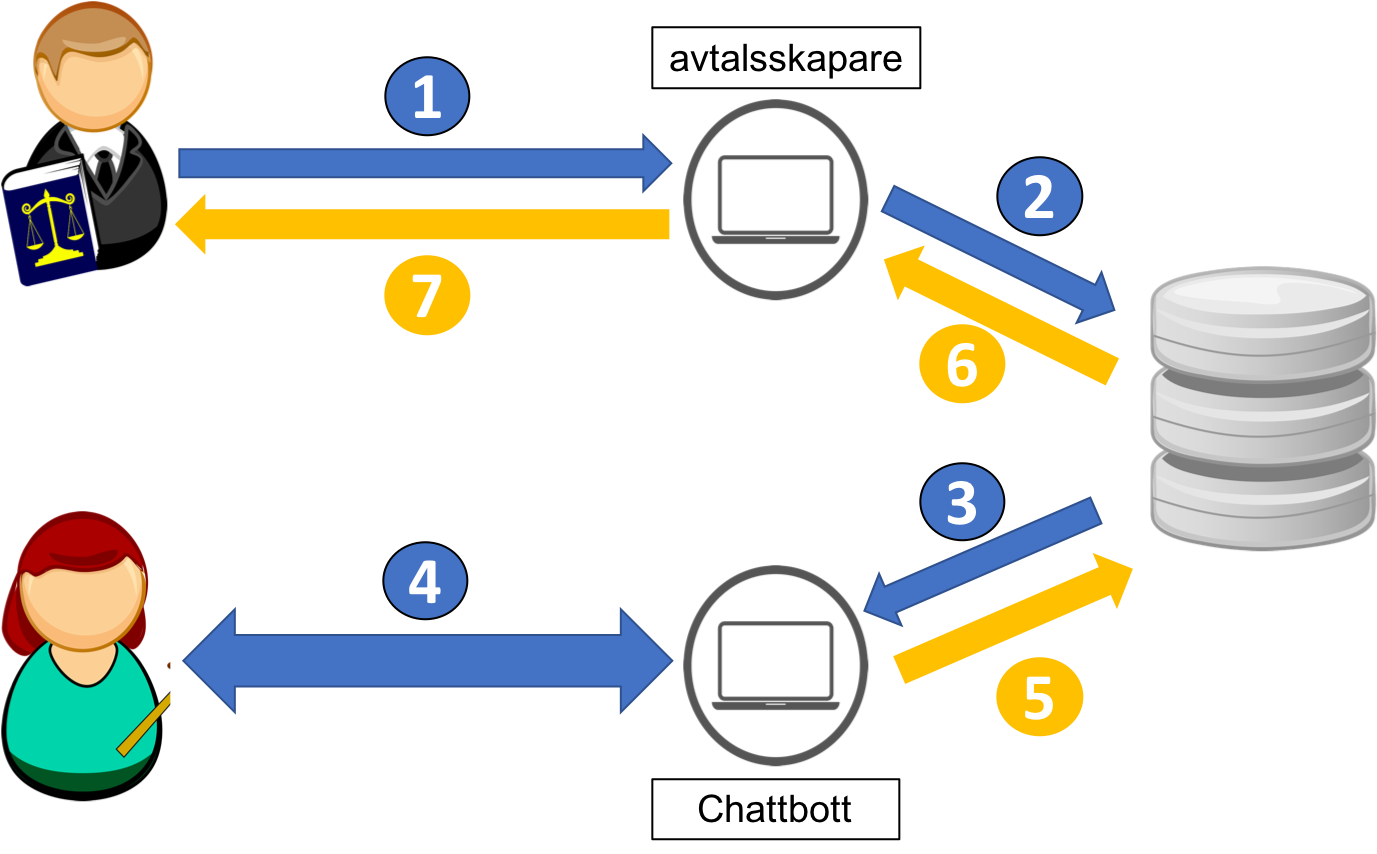
\includegraphics[width=0.8\textwidth,trim={0cm 0cm 0cm 0cm},clip]{img/systemobersikt.png}
    \caption[LoF entry]{Översiktligt diagram av relation mellan målgrupperna och systemet. 
    %Gubben med an lagbok ska föreställa juristgruppen, kvinnan ska föreställa en kundgruppen och de staplade diskarna representerar systemets databas. 
    (1) En jurist skapar via avtalsskaparen en avtalsmall, till exempel en mall för ett samboavtal. (2) Efter att mallen skapas sparas den i databasen. (3) Databasen gör den nya mallen tillgänglig för chattbotten. (4) Via chattdialog med användare kan en mall fyllas i. (5) När användare fyllt i ett helt avtal sparas dess svar i databasen. (6) När databasen erhållit de nya svaren för avtalet uppdateras en lista hos avtalsskaparen som innehåller alla ifyllda avtal. (7) En jurist kan nu granska avtalet och slutföra processen.
    
    % vill ha mer spacing :( space vill inte
    %\makebox[\linewidth]{}
    \vspace{0.8ex}
    \makebox[\linewidth][r]{Bilder hämtade från \textit{\url{https://pixabay.com}}}
    }
    \label{fig:target-group-relation}
\end{figure}

Systemet har två målgrupper: jurister och kunder. Juristerna är de med tillräcklig kunskap för att kunna skapa avtal och kunderna är de som vill teckna ett avtal eller få hjälp med att hitta rätt avtal att teckna, alltså privatpersoner.

Varje målgrupp har ett eget användargränssnitt till systemet för att kunna utföra den målgruppens roll. Juristerna ska använda gränssnittet som kallas för administratörs\-verktyget. I detta gränssnitt kan juristerna skapa mallar för olika avtal, som kunderna senare kan fylla i.

Den andra målgruppen, kunderna, har tillgång till ett annat gränssnitt som endast innehåller ett chattfönster. I detta fönster kan kunden föra en konversation med en chattbott för att först ta reda på vilket av juristens tidigare skapade avtal som ska fyllas i. Därefter kan kunden fylla i avtalet genom att svara på frågorna i avtalets avtalsmall. 

\section{Relaterat arbete}
\label{sec:related-work}
I projektet analyserades andra system som implementerat en chattbott och en avtalsskapare. Vi kommer diskutera och jämföra dels vilket djup de relaterade arbetens chattbott har i sin utformning och hur avtal hanteras. Som grund jämför vi med vårt system som består av komponenterna: en chattbott för kund och en avtalsskapare för administratör. 

%Vidare kommer de två huvudområden för programmering av chattbottar, AI- och regelbaserad, diskuteras och med motivation till varför det här projektet använder sig av en AI-baserad chattbott.
 
\subsection{Liknande system}
\label{subsec:similair-sys}
Automatisering av tidskrävande och standardiserade avtal är ingenting nytt, exempel på existerande system är Automio och DoNotPay~\cite{web:automio, web:donotpay}. De nämnda systemen bistår, i olika utsträckning, användaren med behandling av juridiska dokument. Skillnader och detaljer rörande respektive systemen följer nedan.
\subsubsection{Automio}
Automio lanserades 2017 och syftar till att effektivisera repetitiva dokumentationstjänster. Automio är uppbyggt på en tjänst som skapar ett flöde av frågor kopplat till ett specifik avtal framtaget av en jurist. Vid användande av systemet lagras varje svar och när samtliga frågor är besvarade sammanställs ett avtal med alla svar inlagda~\cite{web:law-society-Automio}.

Automios relation till detta projekt är dess behandling av automatisering och effektivisering av avtalshantering. Varje flöde av frågor är anknutet till ett specifikt avtal. Vidare är Automio utformat på ett sådant sätt att ifrån utgångsläget måste användaren explicit välja vad för avtal som ska fyllas i. Det krävs alltså att användaren på förhand är införstådd med vilket avtal denne vill teckna. Det här innebär en markant skillnad mellan Automio och vårt system. Vårt system genomför istället en kontinuerlig tolkning av kundens avsikt via chattdialogen för att därefter automatiskt ta fram korrekt avtal som kunden vill teckna. Detta beskrivs ytterligare under rubrik~\ref{subsec:IBM-watson-ass}.


%VIDARE BESKRIVNING AV FLÖDET/BESKRIVNING AV AUTOMIOS DOKUMENTATIONS FÖRSÄLJNINGSTJÄNST

\subsubsection{DoNotPay}
DoNotPay lanserades 2017~\cite{web:daily-mail-DoNotPay}. Systemet har en enkel och väldigt specifik inriktning i dess grundutformning, den bestrider parkeringsböter. Med grundutformning menas dess originella funktionalitet som systemet hade 2017. 2018 påbörjades en stor och övergripande uppdatering av hela systemet för att möjliggöra för användaren att bestrida mer än bara parkeringsböter~\cite{web:motherboard-DoNotPay}. 

I grundutformingen, alltså  bestridandet av parkeringsböter, hjälper systemet en anv\-ändare att bestrida en parkeringsbot genom att en chattbott ställer ett antal frågor och registrerar svaren. Tjänsten kräver att användare initialt väljer typ av parkeringsbot och geografiskt område, liknande Automio. Systemet använder en chattbott vars beteende kan beskrivas som ett frågeformulär i form av ett chattgränssnitt.

Efter att DoNotPay erhållit initialvärden sker en dialog med chattbotten, som har ett antal förgenererade svar för de frågor som inte är kopplade till ett direkt bestridande. Systemet registrerar de svar användaren anger, oavsett om de faktiskt innehåller den information som efterfrågas eller inte~\cite{web:pennyhoarder-DoNotPay}.

Ett exempel, om chattbotten frågar efter en adress och användaren svarar med ett klockslag kommer systemet att acceptera svaret. Likväl när systemet efterfrågar ID-numret på en parkeringsbott sker ingen kontroll att det är ett giltigt nummer. %I motsats kommer dialogen med chattbotten för vårt system kontrollera att formatet på svaret stämmer överens med vad som förväntas i den juridiska handlingen. 

DoNotPay har inte en dialog med användaren utan är ett mer utvecklat frågeformulär varifrån felaktig eller inkorrekt inmatning inte kan ändras utan processen måste börjas om. Vårt system fungera annorlunda jämfört med DoNotPay då vårt system frågar användaren via chattbotten vilket avtal som ska fyllas i, istället för att fylla i kryssrutor innan dialogen som DoNotPay gör. Vårt system kommer även att kolla om de inmatade svaren är på rätt format eller av rätt sort och kommer att fråga om frågan om de inte är det.

% Robot Lawyer Lisa utveckla mer

%\subsection{AI- kontra Regelbaserad chattbott} \label{sec:egenskapar-hos-chatbottar}

%I detta avsnitt kommer en chattbott som har NLP och AI-kapacitet att jämföras med en chattbott som är regelbaserad. För den NLP-baserade chattbotten kan svaret ``Ja'' tolkas som en avsikt att svara ja på en fråga, med möjlighet att även tolka synonymsvar som ``absolut, yep, kör hårt, det godtar jag'' som ett ja på grund av NLP:en. Medan ett regelbaserat system måste svaren vara explicit bestämda av programmeraren, om ``yep'' inte har programmerats som svar på frågan kommer systemet inte heller tolka det som ett ja. Det kan bli en skillnad om det regelbaserade systemet har en NLP. Med en NLP kommer det regelbaserade systemet ha en större felmarginal när den tolkar ett svar. Överlag är en NLP ett väldigt bra inslag i en chattbott då det kan bidra till känslan att användaren samtalar med en människa~\cite{web:chatbotmagazine-paul-boutin}. 

%I projektet är det väsentligt att tolka kundens svar, utifrån perspektivet vad kunden har för avsikt snarare än att enbart reagera utifrån vad som skrivits. Som exempel, om systemet enbart låter en kund teckna samboavtal om ordet `samboavtal' explicit skrivs i chattdialogen motverkas syftet med projektet. Tillåts systemet istället tolka texten `jag vill flytta ihop med min respektive' som en avsikt att flytta ihop blir systemet inte bara effektivare utan också lättare att använda. 

%Som nämns i syftet under rubrik~\ref{sec:syfte} kan juridiska termer ofta vara invecklade och svårförståeliga. En chattbott som kontinuerligt lär sig och utvecklas, vilket är möjligt med en AI uppbyggd NLP, och kan förstå vad kunden vill kan därmed blir både effektivare, mer verklighetstrogen och bättre bistå en kund. Utifrån detta dras slutsatsen att vi vill använda en AI-baserad chattbott med NLP.

\section{Metod}
{\em
%Här beskriver ni vilka metoder/verktyg/tekniker/approacher ni använt för att lösa problemet / besvara frågeställningen.  Vilka metoder har ni konkret använt för att lösa problemet/bygga systemet?  Vilka tekniker/verktyg använde ni? Observera att det inte är samma sak som att beskriva \emph{hur} ni använde teknikerna/verktygen (det kommer i Del X).

%Glöm inte att \emph{motivera} era val av metoder. Finns det flera rimliga alternativ? Beskriv varför ni inte valt dem (t.ex.~varför er valda metod är bättre).
%Visa att det är rimligt att använda just detta tillvägagångssätt.

%Detta avsnitt ska \emph{inte} innehålla in formation om hur gruppen organiserat arbetet (github, trello\ldots) \emph{om} det inte är relevant för resultatet (och det är det oftast inte).
}
%Projektet består av ett antal komponenter: IBM Watson Assistant, React.js för klientsidan, node.js för serversidan och MySQL som databas. I det här avsnittet kommer varje komponent att diskuteras och jämföras med alternativ.

I det här avsnittet beskrivs, diskuteras och jämförs vilka metoder vi har använt. Sammanfattningsvist använde vi IBM Watson Assistant som tjänst för att tolka indata från användarna, React.js för att göra gränssnittet på webbsidorna, node.js för att driva servern och till sist MySQL som vår databas.

Efter en litteraturstudie där vi jämförde Watson med ett antal alternativ (mer om detta under rubrik~\ref{sec:alternativa:chattbottar}) valde vi att använda Watson. Efter det initiala planeringsarbetet av projektet och en plan för de olika komponenterna som behövdes i projektet (se systemstruktur avsnitt~\ref{sec:systemstruktur}) följde en designfas för chattgränssnitt och avtalsskaparen. När designfasen var avslutad och internt testad påbörjades en utvecklingsperiod med dagliga möten som hjälpte gruppen framåt och gjorde att vi kunde säkerställa att inget släpade efter.
%De metoder vi använde oss av för utveckling av systemet beskrivs i följande avsnitt.

\subsection{Chattbottar}

Under denna rubrik diskuteras två olika kategorier av chattbottar samt förklaringar av IBM Watson Assistant i detalj och kort om dess alternativ.

\subsubsection{AI-chattbottar och regelbaserade chattbottar}
\label{sec:ai:vs:regel}

I detta avsnitt kommer en chattbott som har NLP och AI-kapacitet att jämföras med en chattbott som är regelbaserad. För den NLP-baserade chattbotten kan svaret ``Ja'' tolkas som en avsikt att svara ja på en fråga, med möjlighet att även tolka synonymsvar som ``absolut, yep, kör hårt, det godtar jag'' som ett ja på grund av NLP:en. Medan ett regelbaserat system måste svaren vara explicit bestämda av programmeraren, om ``yep'' inte har programmerats som svar på frågan kommer systemet inte heller tolka det som ett ja. Det kan bli en skillnad om det regelbaserade systemet har en NLP. Med en NLP kommer det regelbaserade systemet ha en större felmarginal när den tolkar ett svar. Överlag är en NLP ett väldigt bra inslag i en chattbott då det kan bidra till känslan att användaren samtalar med en människa~\cite{web:chatbotmagazine-paul-boutin}. 

I projektet är det väsentligt att tolka kundens svar, utifrån perspektivet vad kunden har för avsikt snarare än att enbart reagera utifrån vad som skrivits. Som exempel, om systemet enbart låter en kund teckna samboavtal om ordet `samboavtal' explicit skrivs i chattdialogen motverkas syftet med projektet. Tillåts systemet istället tolka texten `jag vill flytta ihop med min respektive' som en avsikt att flytta ihop blir systemet inte bara effektivare utan också lättare att använda. 

Som nämns i syftet under rubrik~\ref{sec:syfte} kan juridiska termer ofta vara invecklade och svår\-förståe\-liga. En chattbott som kontinuerligt lär sig och utvecklas, vilket är möjligt med en AI uppbyggd NLP, och kan förstå vad kunden vill kan därmed blir effektivare, mer verklighetstrogen och kan bättre bistå en kund. Utifrån detta dras slutsatsen att vi vill använda en AI-baserad chattbott med NLP.

\subsubsection{IBM Watson Assistant}
\label{subsec:IBM-watson-ass}
\FloatBarrier

\begin{figure}[htb]
  \centering
  \smallskip
  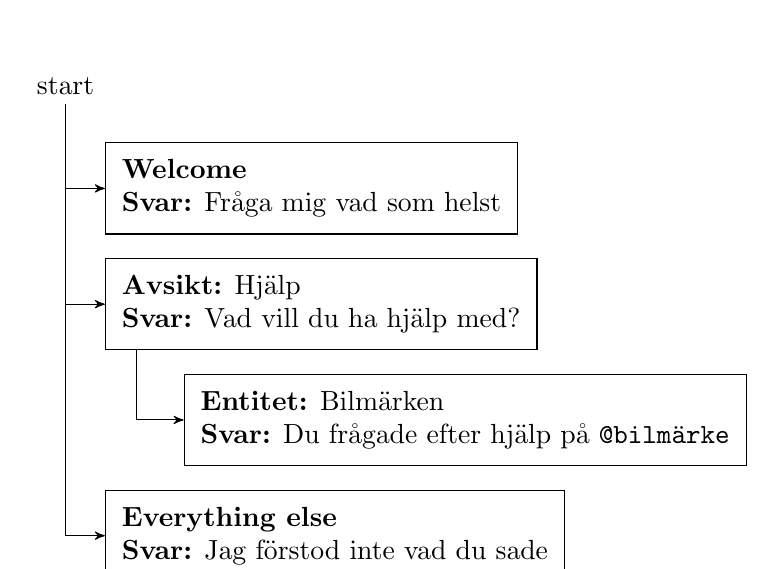
\begin{tikzpicture}[
    rekt/.style={rectangle,draw,inner sep=6pt,anchor=north west,align=left}
  ]
    \node (N0) at (0,0) [rekt] {\textbf{Welcome}\\\textbf{Svar:} Fråga mig vad som helst};
    \node (N1) at ($(N0.south west) + (0, -0.3)$) [rekt] {\textbf{Avsikt:} Hjälp\\\textbf{Svar:} Vad vill du ha hjälp med?};
    \node (N11) at ($(N1.south west) +(1, -0.3)$) [rekt] {\textbf{Entitet:} Bilmärken\\\textbf{Svar:} Du frågade efter hjälp på \texttt{@bilmärke}};
    \node (ROOT) at ($(N0.west) + (-0.5,1.3)$) {start};
    \draw let 
            \p1 = (N1.west),
            \p2 = (N11.south)
        in
            node [rekt] (N2) at ($(\x1,\y2) + (0,-0.3)$) {\textbf{Everything else}\\\textbf{Svar:} Jag förstod inte vad du sade};
            
    \draw[->] (ROOT) |- (N0.west);
    \draw[->] (ROOT) |- (N1.west);
    \draw[->] (N1.south west) +(0.4, 0) |- (N11.west);
    \draw[->] (ROOT) |- (N2.west);

  \end{tikzpicture}
  \smallskip
  \caption{Watson Assistant dialogträd}
  \label{fig:watson:dialog-tree}
\end{figure}

Vi har valt att använda IBM Watson Assistant till detta projekt.
Watson Assistant är en molntjänst, utvecklad av IBM~\cite{web:watson-assistant}. Det är AI-baserad chattbott som kan lära sig att förstå och tolka bättre vad användarna skriver (se rubrik~\ref{sec:sprakteknologi}). Watsons förmåga att tolka meningar grundar sig i \emph{avsikter} och \emph{entiteter}.

\begin{itemize}
    \item En \textbf{avsikt} är vad vi vill att Watson ska förstå. För att lära Watson innebörden av en sådan ges exempel på svar som en användare kan tänkas skriva. Exempelvis för att lära Watson hur den vet om en användare vill ha hjälp kan exempelsvaren vara: ``jag behöver hjälp'' och ``jag kan inte själv''.
    
    \item Ett \textbf{entitet} är ett objekt i en sats som en användare kan prata om. Till exempel kan Watson lära sig om bilmärken. Om en användare nämner ett bilmärke i konversationen kommer Watson att se det och extrahera ut och eventuellt spara det värdet.
\end{itemize}
Watson kommer sedan, med hjälp av dessa entiteter och avsikter, att bygga en maskininlärningsmodell som kan känna igen rätt entiteter och avsikter från andra liknande uttryck till de exempel som definierade dem.

För att få Watson att faktiskt ha en konversation behövs ett dialogträd. Ett exempel på en sådan visas i figur~\ref{fig:watson:dialog-tree}. Det är ett träd där varje nod kan ha flera barnnoder och varje nod innehåller vilken avsikt den ska svara emot och vilken respons den ska ge. Det finns speciella villkor som kan sättas på noder: \emph{Welcome} som är den nod som körs en gång som initialt svar och \emph{Everything else} som kör när ingenting annat passar. 

\FloatBarrier

\begin{figure}[htb] % ska helst sitta ihop eller vara väldigt nära stycket under
  \centering
  \smallskip
  \begin{minipage}{0.7\textwidth}%
    \newcommand{\talktalk}[3]{
        \stepcounter{conversationCounter}
        #1
        \framebox[0.4\linewidth][l]{
            \parbox{0.37\linewidth}{
                {\footnotesize\bfseries #2}\hfill\textcolor{darkgray}{\#\arabic{conversationCounter}}\\#3
            }
        }\par
    }%
    \newcommand{\bottalk}[1]{\talktalk{}{Watson}{#1}}%
    \newcommand{\usertalk}[1]{\talktalk{\hfill}{Användaren}{#1}}%
    \newcounter{conversationCounter}
    \bottalk{Fråga mig vad som helst}
    \usertalk{hjälp}
    \bottalk{Vad vill du ha hjälp med?}
    \usertalk{Volvo}
    \bottalk{Du frågade efter hjälp på en Volvo}
    \usertalk{kan du några skämt?}
    \bottalk{Jag förstod inte vad du sade}
  \end{minipage}\smallskip
  \caption{Exempel på en konversation med figur~\ref{fig:watson:dialog-tree}.}
  \label{fig:watson:example}
\end{figure}

En exempelkörning av trädet i figur~\ref{fig:watson:dialog-tree} visas i figur~\ref{fig:watson:example}. Där börjar konversationen i start med att Watson skriver ut det som står i welcome-noden (\#1). Användaren skriver sedan ``hjälp'' (\#2) varav Watson ser att det finns en nod som passar på avsikten för hjälp. Watson skriver ut svaret som står i den noden och väntar nu där (\#3). Detta betyder att barnen till den noden kommer testas först till nästa svar som användaren skriver. Om inget där passar kommer Watson att gå tillbaka till start och kolla om någon nod passar där. Om inget passar där heller kommer inget svar att skrivas ut. I det här fallet finns en ``Everything else'' som alltid matchar, vilket betyder att någonting alltid kommer att skrivas ut.

Användaren fortsätter med att skriva bilmärket ``Volvo'' (\#4), Watson ser att ``volvo'' är ett bilmärke och skriver ut det som står i den matchande noden. Svaret på den noden är speciellt då den refererar mot den entitet som matchades. Detta betyder att Watson inkluderar svaret från användaren i \#4 i sitt egna svar (\#5).

Nu finns det inga fler barnnoder vilket betyder att Watson hoppar tillbaka till start och väntar på mer indata från användaren. Denna gång skriver användaren någonting som inte passar in i någon specifik nod (\#6), vilket gör att fallback-noden matchas (\#7).

Nu börjar allt om igen i start och konversationen kan fortsätta.

\FloatBarrier

\subsubsection{Alternativa chattbottsystem}
\label{sec:alternativa:chattbottar}

På grund av det som diskuterades under rubrik~\ref{sec:ai:vs:regel} är det endast AI-chattbottar som är av intresse. Därav finns minst två intressanta alternativ till IBM Watson Assistant: wit.ai och Dialogflow.

\paragraph{Wit.ai} Wit.ai är en AI-chattbott som är mer öppen än IBM Watson då den delar alla \emph{avsikter} och \emph{entiteter} publikt till alla~\cite{web:witai}. Den gör detta för att lära sig från alla som använder tjänsten, alltså hjälper alla användare varandra. Den använder sig av \emph{entiteter} och \emph{avsikter} på precis samma sätt som IBM Watson. Wit.ai har dock inte något dialogträd, den analyserar bara text för att hitta \emph{avsikter} och \emph{entiteter}.

\paragraph{Dialogflow} Dialogflow är en tjänst av Google som också är en AI-chattbott~\cite{web:dialogflow}. Precis som wit.ai och IBM Watson analyserar denna \emph{avsikter} och \emph{entiteter}. Dialogflow är som IBM Watson också en betaltjänst, men använder Agents istället för dialogträd. Dessa Agents är listor av \emph{avsikter} och fungerar som dialogträd fast utan barnnoder.

\emptyparagraph Vi har valt IBM Watson framför dessa alternativ för att Watson har ett dialogträd. Eftersom att chattbotten i detta projekt kommer att ställa många frågor efter varandra är ett dialogträd att föredra då det enkelt kan skapas följdfrågor genom barnnoder (se exemplet i figur~\ref{fig:watson:example}). Att använda dialogträd är ett passande sätt att strukturera upp chattbottens konversation, då dialogträdet som modell för en dialog stämmer väl överens med verkligheten.

\subsection{Node.js}
\label{sec:nodejs}
\FloatBarrier
För att driva servern används Node.js, vilket är en asynkroniskt händelsestyrd exekveringsmiljö för Javascript~\cite{web:nodejs}. Med detta menas att Node.js använder callback-\-funktioner istället för trådar och event-loopar\footnote{Node.js egna interna event-loop är inte den som menas här, utan de som programmeraren måste göra själv}. En callback-funktion är en funktion som ska köras när en händelse sker. Exempel på händelser är när någon ansluter till node eller om en timer avfyras. I figur~\ref{fig:node:callback} visas ett exempel på en callback-funktion som körs varje gång ett HTTP-anrop tas emot.

Fördelen med att det är designat att bara ha callback-funktioner är att det blir enklare att hantera flera anslutningar samtidigt~\cite{web:nodejs}. Istället för att göra en ny tråd för varje anslutning körs istället den callback som specificerats att köra på nya anslutningar. Det blir enklare för att den trådfria designen tar bort risken för deadlocks då behovet av lås försvinner~\cite{web:nodejs, web:wikipedia:deadlock}. 

\begin{figure}[htbp]
    \centering
    \begin{lstlisting}[language=jsx]
const server = http.createServer(function(req, res) {
  res.statusCode = 200;
  res.setHeader('Content-Type', 'text/plain');
  res.end('Hej\n');
});
server.listen(3000, '127.0.0.1');
    \end{lstlisting}
    \caption{Ett exempel på en callback-funktion. Meddelandet ``Hej'' skickas tillbaka varje gång någon gör en HTTP-anrop till servern.}
    \label{fig:node:callback}
\end{figure}

Den huvudsakliga anledningen till valet av Node.js är att programmeringsspråket den tolkar är javascript, vilket är samma språk som stöds och används i de flesta webbläsare för att göra webbsidan interaktiv~\cite{web:mozilla:whatisjs}. Fördelen med att ha samma språk både på klientsidan och serversidan är att bland annat datastrukturer inte behöver översättas för att kunna användas mellan två olika programmeringsspråk.

\FloatBarrier

%\subsubsection{Alternativ och motivation till Node.js}
%\paragraph{Twisted}
%Twisted~\cite{twisted} är ett asynkroniskt och händelsestyrt ramverk skrivet i Python. Python är ett väletablerat och platformsöverskriddande programmeringsspråk men, som beskrivs tidigare under~\ref{sec:nodejs} uppstår då potentiellt ett problem med översättning mellan programmeringsspråk.

%Den primära anledningen för att Twisted inte nyttjas till det här projektet är dels att vi vill undvika att använda olika programmeringsspråk på frontend respektive backend, och vanan sedan tidigare att använda Node.js.

%eventmachine
%PHP

\subsection{React.js}
\label{subsec:react}
\FloatBarrier
React är ett javascript-ramverk utvecklat av Facebook~\cite{web:react}. Detta ramverk är till för att bygga så kallade ``single-page applications'' vilket är webbsidor som laddar endast en HTML-fil och uppdaterar den dynamiskt~\cite{web:wikipedia:spa}. Eftersom sidan uppdateras dynamiskt laddas inte sidan om då när vyn byts till en undersida, utan endast de relevanta bitarna laddas in.

En webbsida i React är uppbyggd av komponenter och varje komponent beskriver hur den själv ska renderas på webbsidan~\cite{web:react}. I figur~\ref{lst:react:basic} på rad~\ref{lst:react:basic:class} finner vi ett exempel på en komponent implementerat som en klass. Denna klass har en metod \li{render} som returnerar vad som ska visas. I det här fallet ska en \li{div} med innehållet av argumentet \li{name} visas i en \li{p}-tagg. Observera att en komponent endast kan bestå av en tagg. Den taggen kan innehålla hur många barntaggar den vill men render-metoden får bara returnera en tagg. För att rendera en komponent på webbsidan används funktionen \li{ReactDOM.render} (på rad~\ref{lst:react:basic:render}), denna tar som argument vilken React-komponent som ska renderas och vart på HTML-sidan den ska renderas. Observera att det är här på rad~\ref{lst:react:basic:name} som name-argumentet till komponenten specificeras.

\begin{figure}[htbp]
\centering
\begin{lstlisting}[language=jsx,morekeywords={[3]<HelloMessage}]
class HelloMessage extends React.Component {|\label{lst:react:basic:class}|
  render() {
    return (
      <div>
        <p>||Hello {this.props.name}</p>
      </div>
    );
  }
}

ReactDOM.render(|\label{lst:react:basic:render}|
  <HelloMessage name="Taylor" />,|\label{lst:react:basic:name}|
  document.getElementById('hello-example')
);
\end{lstlisting}
\caption{En enkel React-komponent}
\label{lst:react:basic}
\end{figure}

Att varje komponent beskriver hur den vill renderas istället för att göra det själv instruktion för instruktion kallas för deklarativ programmering~\cite{web:wikipedia:declarative}. Hur komponenten renderas och vilka som renderas ansvarar React för. Till exempel om \li{name} i figur~\ref{lst:react:basic} på rad~\ref{lst:react:basic:name} ändrades till \li[language=jsx]{"Kalle"} skulle React jämföra den gamla HTML-strukturen med det nya för att komma fram till att endast \li{p}-taggen behöver ändras och låter \li{div}-taggen vara kvar som den är~\cite{web:react}. Den dynamiska uppdateringen är en av fördelarna och en av anledningarna till att vi valde React.

Valet att använda React föll på att det var ett av de populäraste ramverken vid rapportens skrivande och att det därför skulle vara bra att lära sig.
\FloatBarrier

\subsection{MySQL}
\label{sec:sql}
MySQL är en relationsdatabashanterare där all data organiseras i tabeller. För att kommunicera med en MySQL-databasen används SQL (Structured Query Language)~\cite{web:MySQL}. I SQL-tabeller måste alla element i varje kolumn (fält) vara av samma datatyp och antalet kolumner får inte ändras. Dessa två restriktioner gör att tabellerna inte är flexibla.

För att organisera SQL-tabeller kan man lägga till vissa fält som är speciella. En av dessa är \mbox{\textbf{primary key}} (PK), vilket är ett fält vars värden måste vara unika inom tabellen. Att hämta rätt rad ur tabellen underlättas om det finns ett värde som är garanterat att vara unikt för den raden. Ett annat speciellt fält som finns är \mbox{\textbf{foreign key}} (FK), vilket används för att koppla ihop tabeller. Att ett fält i en tabell är en FK mot ett fält i en annan tabell betyder att värdena i den första tabellen endast får bestå av värden som finns i den andra tabellen. Kopplingen uppnås genom att en tabell refererar till en PK i en annan tabell.

% ett exempel vore sugoi

Eftersom vår data är strukturerad (inte flexibel) passar det bra att organisera den i tabeller, MySQL valdes av denna anledning.

%Våra krav på en databashanterare var att kunna spara data på ett strukturerat sätt och hämta data på ett effektivt sätt. MySQL uppfyllde dessa krav vi hade på en databashanterare samt så hade vi redan kompetens om MySQL inom gruppen vilket bidrog till att valet föll på MySQL.

    %Som alternativ till MySQL finns till exempel MongoDB. MongoDB spara datan i flexibla json-liknande dokument, vilket betyder att man inte är begränsad till fördefinerade tabeller att lagra data i~\cite{web:MongoDB}.

%Andra lämpliga databashanterare var PostgreSQL
% spara och hämta data, inga dups, 
%Vi kan MySQL och den täckte våra behov
%Andra så som PostgreSQL och mongoDB kunde ha varit lämpligare, men erfarenhet inom MySQL

\section{Systemstruktur}
\label{sec:systemstruktur}
%\begin{figure}
%\begin{center}
%  
\includegraphics[height=5\baselineskip]{logo_name.pdf}
%\hspace{2cm}
%  
\includegraphics[height=5\baselineskip]{logo_name_sv.pdf}
%\end{center}
%\caption{Till vänster syns universitetets logotyp i färg, till höger i svartvitt.}
%  \label{fig:exempel}
%\end{figure}

%{\em
%Beskriv strukturen både internt (hur ert eget system är uppbyggt) och externt (vilka andra system ert system kommunicerar med). \textbf{Använd figurer} (och text)!
%\begin{itemize}
%\item Vilka delar består systemet av? (T.ex. databas, webbinterface, AI-modul, grafik...) Vilka kommunicerar med vilka, beror av vilka, innehåller vilka andra?
%\item Vilka delar fanns färdiga att använda/anpassa, vilka utvecklade ni själva? Visa tydligt, gärna grafiskt.
%\item Finns olika alternativa byggblock eller designval? Vilka är argumenten för/emot valen?
%\item Hur kommunicerar delarna, vilka protokoll och/eller dataformat används? (Beskriv mer detaljerat i senare, i Huvuddelen.)
%\item Finns det olika typer av användare/motsv? (T.ex. administratörer resp slut\-an\-vän\-dare?)
%\end{itemize}
%}

\newcommand{\doublearrow}[4][0]{%
\draw ($#2 + (-#4, -#1)$) edge[->] ($#3 + (-#4, -#1)$)
      ($#3 + (#4, #1)$)   edge[->] ($#2 + (#4, #1)$);
}
\begin{figure}[H]
  \centering
  \smallskip
  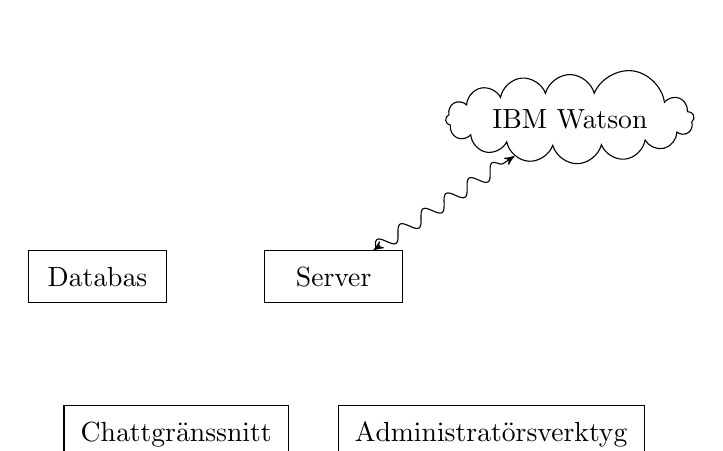
\begin{tikzpicture}[rekt/.style={rectangle,draw,inner sep=6pt, minimum width=50pt}]
    \node (CLNT) at (-2,0) [rekt] {Chattgränssnitt};
    \node (NDJS) at (0,2) [rekt] {Server};
    \node (SQL)  at (-3, 2) [rekt] {Databas};
    \node (CREA) at (2, 0) [rekt] {Administratörsverktyg};
    
    \doublearrow{(CLNT.north)}{(NDJS.south) + (-0.3, 0)}{0.3}
    \doublearrow{(NDJS.south) + (0.3, 0)}{(CREA.north)}{0.3}
    \doublearrow[1ex]{(SQL.east)}{(NDJS.west)}{0}
        
    \node (IBW) at (3, 4)
        [cloud,
         cloud puffs=15.7,
         cloud ignores aspect,
         minimum width=50pt,
         minimum height=0pt,
         draw
        ] {IBM Watson};
        
    \draw[<->,decorate,decoration=snake]
        (NDJS) -- (IBW);
  \end{tikzpicture}
  \smallskip
  \caption{Diagram över systemstrukturen}
  \label{fig:system:structure}
\end{figure}

I figur~\ref{fig:system:structure} finner vi en teknisk överblick av systemet. Den består av fem moduler: ett chattgränssnitt, ett administratörsverktyg, en server, en databas, och en extern tjänst IBM Watson Assistant.

Chattgränssnitt är den modul där en kund söker juridisk rådgivning genom att skriva med chattbotten. Gränssnittet är en webbsida gjord med React.js och kommunicerar med servern via WebSockets och HTTP-anrop.

Modulen administratörsverktyget är den modul där juristen skapar avtalen som anv\-ändaren kan fylla i. Denna modul är också gjord i React.js och kommunicerar med servern på samma sätt som användaren. Avtal som skapas här lagras i databasen tillsammans med svaren från ifyllda avtal.

Servern är utvecklad med Node.js och det är där den mesta logiken sker. Som går att utläsa ur figur~\ref{fig:system:structure} sammankopplar servern samtliga komponenter och koordinerar dem. För att använda IBM:s-molntjänster gör servern API-anrop till IBM med hjälp av HTTP-anrop, det som skickas i dessa anrop är JSON-objekt.

Ett typiskt dataflöde när en kund skriver med chattbotten är följande:
\begin{enumerate}
    \item\label{sysstruct:dataflow:1} Kunden skriver ett meddelande i gränssnittet och meddelandet skickas till servern.
    \item Servern skickar meddelandet till IBM Watson som tolkar det och skickar tillbaka ett svar.
    \item Om det är ett avtal som fylls i avgör servern om detta avtal är ifyllt eller inte.
      \begin{enumerate}[a)]
            \item \textbf{Om ifyllt:} sparar servern de ifyllda svaren i databasen.
            \item \textbf{Om inte:} fortsätter konversationen.
        \end{enumerate}
    \item Servern skickar sedan svaret till användaren.
    \item Börja om i punkt~\ref{sysstruct:dataflow:1}.
\end{enumerate}

\subsection{Designval}

Här beskrivs de större val vi gjorde i designen av systemet och varför vi valt att utforma delar av systemet på ett visst sätt.

\subsubsection{Behovet av en server} 

Mycket av logiken från servermodulen går att flytta till chattgränssnittet och nästan eliminera behovet av servern helt (webbsidan måste kommas åt på något sätt fortfarande). En nackdel med att låta chattgränssnittet ta över all logik är att det inte är lika tydligt vad för roll varje modul har i systemet. Chattgränssnittets roll är att representera ett gränssnitt för kunden och servermodulens roll är att hantera den bakomliggande logiken och kommunikationen mellan de olika modulerna. Genom att modularisera systemet kan ändringar göras på en modul utan att påverka, eller ha kunskap av, hur en annan modul fungerar. Kodseperation är gynnsamt då kod som inte har modifierats har mindre risk att sluta fungera än kod som har modifierats. 

En annan nackdel med att flytta serverlogiken till chattgränssnittet är att information som bör hållas hemligt från kunden blir tillgängligt i klartext i en javascript-fil. Informationen kan vara sådant som API-nycklar och databaslösenord. Genom att separera servern och användaren är det möjligt att kontrollera vad för information som finns på chattgränssnittet. Samtidigt som den känsliga informationen som databaslösenord kan sparas på servern, där ingen utomstående har åtkomst till det. Om användaren behöver göra något med den känsliga informationen får användaren skicka ett anrop till servern för att få den att hantera det. Till exempel kan användaren skicka anropet “hämta alla avtal” till servern varefter den använder det hemliga databaslösenordet för att hämta alla avtal och skickar dem till chattgränssnittet.

\subsubsection{Val av Dialogträd} Antingen skulle dialogträdet hos Watson kunna nyttjas eller göra ett eget. Att använda det hos Watson betyder att servern blir en mellanhand som bara vidarebefordrar meddelandena mellan klienten och Watson. När ett nytt avtal skapas från avtalsskaparen måste servern utöver att lagra den i databasen också bygga upp dialogträdet på Watson. Detta kräver fler API-anrop, men i utbyte får systemet tillgång till ett redan färdigt dialogträd med mycket funktionalitet.

Att göra dialogträdet själv gör att det går att använda avtalen lagrade i databasen direkt utan att behöva skicka iväg dem till Watson. Men detta skulle kräva mer arbete vilket är anledningen till att vi bestämde oss för att inte göra dialogträdet själva.

%\subsection{Tänk på följande}
%
%Var inte för tekniskt detaljerade här.  Tanken är att ge en översikt över systemet.  Ni behöver inte beskriva objektmetoder etc. i detalj (om de inte är nya och avgörande för resultatet). Tekniska detaljer och implementation beskriver ni snarare i Huvudddelen.
%
%Se till att ni använder \emph{samma terminologi} i figurer som visar systemet som i texten. 
%
%Anknyt figurerna till texten på ett tydligt sätt. Om ni t.ex. har separata underrubriker som beskriver olika delar/aspekter av systemstrukturen med tillhörande figur, välj antingen en underrubrik per del i figuren eller använd helt andra underrubriker.  Annars kommer läsaren att undra var underrubriken som beskriver del X är, när det finns underrubriker för alla andra delar.



\section{Datastruktur för avtalsmallar}
%Mallar skapas med hjälp av ett avtalsmall, vilket är ett sorts dialogträd som är förenklad till att varje nod ställer en fråga och frågan i nästa nod ställs inte förrän frågan i nuvarande nod har besvarats. Anledningen till att det är ett träd och inte en enkel lista är för att vissa frågor kan ha olika följdfrågor baserat på vad svaret är.

% Vad vi ville åstadkomma och varför
En datastruktur för avtalsmallar krävdes för att representera mallarna som dialogträd. Dialogträden användes sedan för att hjälpa chattbotten att leda en konversation med en användare. Konversationens mål är att hitta ett lämpligt avtal och ta fram den nöd\-vändiga informationen som behövs för att kunna fylla i avtalet. 

% -- Implementation
\subsection{Implementation}
\FloatBarrier

\begin{figure}[H]
    \centering
    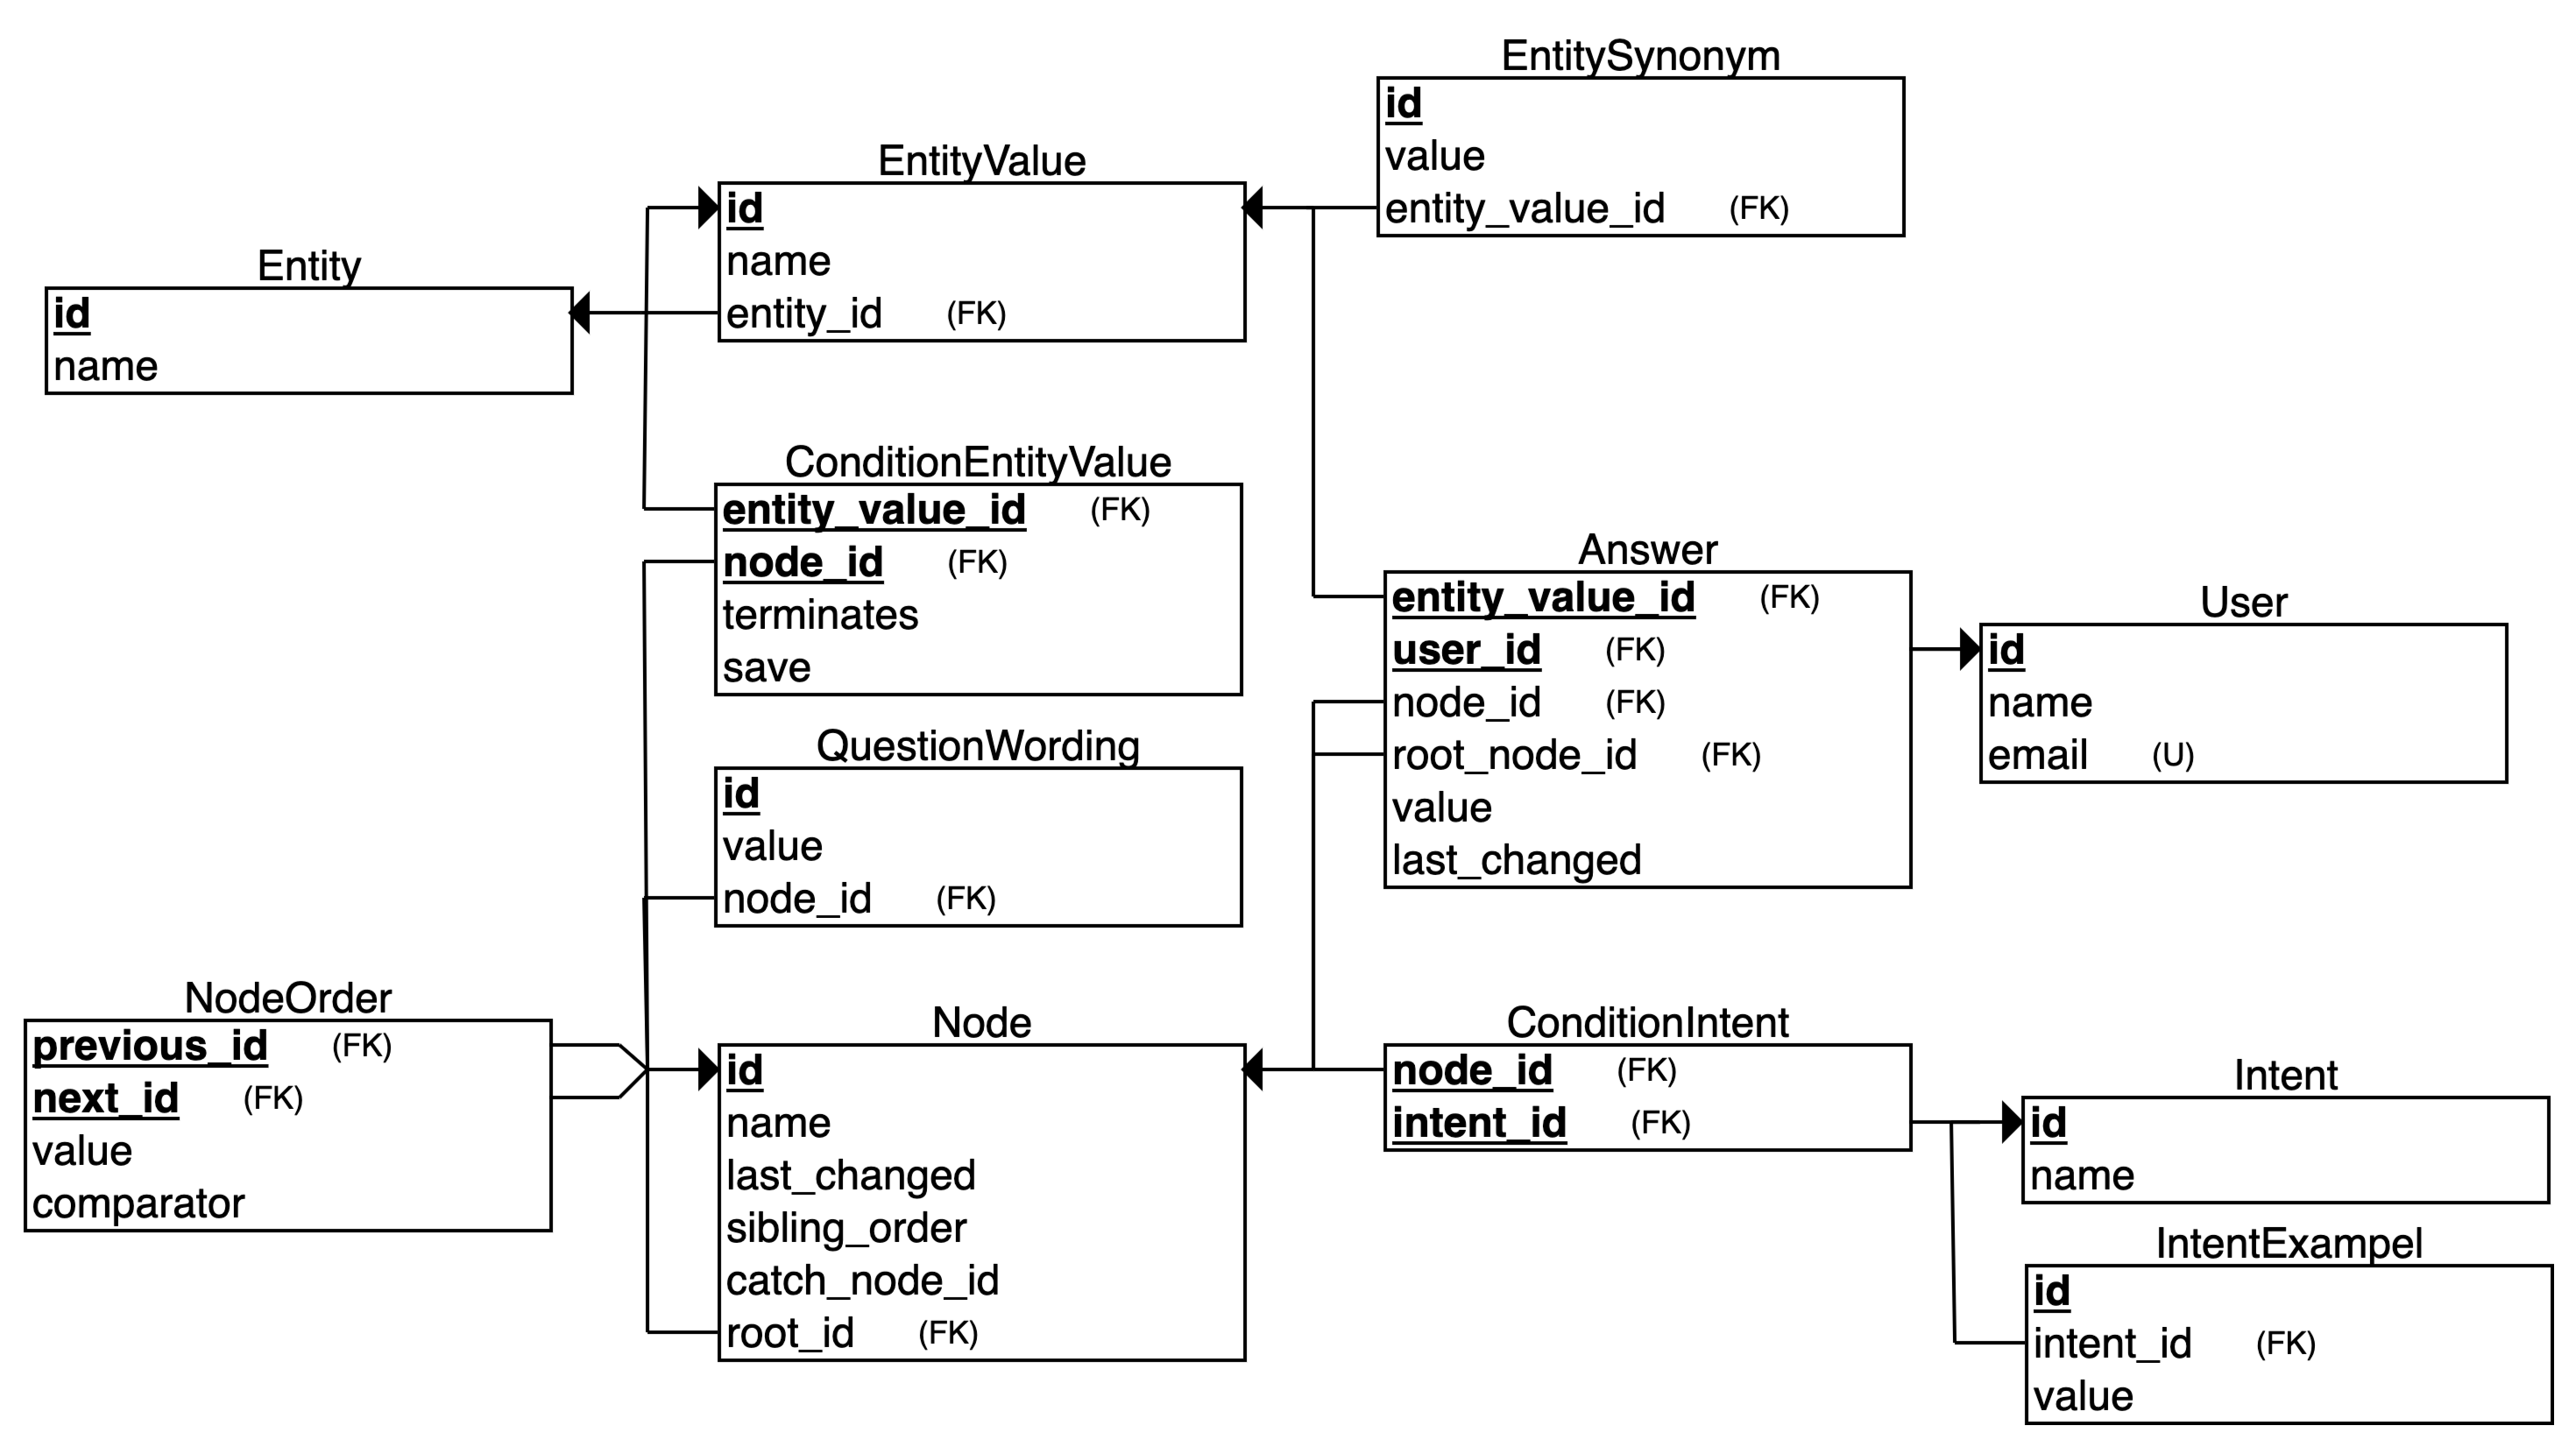
\includegraphics[width=\textwidth]{img/relational.png}
    \caption{Relationsdiagram över SQL-databasen. Rutorna representerar databasens tabeller och varje rad i dessa är namnet på en kolumn. De understrykna fältnamnen representerar att de är en \mbox{\textbf{primary key}} och pilarna representerar att de är \mbox{\textbf{foreign keys}} (se förklaringar under rubrik~\ref{sec:sql}).}
    \label{fig:relation-schema}
\end{figure}

% Noder, Ordning, Skillnad noder och kontrakt
Kontrakt och frågor representeras som noder i dialogträd, och sparas i tabellen \mbox{Node} i figur~\ref{fig:relation-schema}. Frågor har föräldrar för att representera ordningen i trädet, om fråga B har A som förälder kommer A före B i trädet. Ordn\-ingen mellan fråg\-orna sparas i tab\-ellen \mbox{NodeOrder} där \mbox{\emph{previous\_id}} är en referens till föräldern och \mbox{\emph{next\_id}} är en referens till barnet. Skillnaden mellan kontrakt och frågor är att kontrakt inte har någon förälder, de är rotnoderna i alla träd. Rotnoderna används för att gruppera frågor som hör till det kontraktet.

% Intents och entities
För att systemet ska gå in i en specifik nod måste nodens villkor uppfyllas. Villkoret består av avsikter och entiteter och bestämmer vad för indata som förväntas av användaren. Exempelvis kan en nod fråga efter användarens adress och som villkor kräva entiteten adress. Då kommer systemet inte gå vidare till nästa fråga om användaren inte angett en adress, utan ställer om frågan igen tills dess att villkoret uppfyllts. Avsikter och entiteter sparas i tabellerna \mbox{Intent} respektive \mbox{Entity} och kopplas till noder genom tabellerna \mbox{ConditionIntent} och \mbox{ConditionEntityValue}.

\begin{figure}[H]
    \centering
    \smallskip
    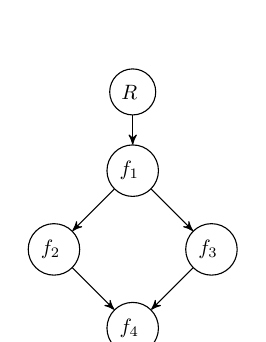
\begin{tikzpicture}[ring/.style={circle,draw=black,align=center,scale=0.75}]
        \node (R) at (0, 0) [ring] { $R$ };
        \node (F1) at (0, -1) [ring] { $f_1$ };
        \node (F2) at (-1, -2) [ring] { $f_2$ };
        \node (F3) at (1, -2) [ring] { $f_3$ };
        \node (F4) at (0, -3) [ring] { $f_4$ };
        
        \draw[->] (R) -- (F1);
        \draw[->] (F1) -- (F2);
        \draw[->] (F1) -- (F3);
        \draw[->] (F2) -- (F4);
        \draw[->] (F3) -- (F4);
    \end{tikzpicture}
    \smallskip
    \caption{Visualisering av nodernas ordning. Rotnoden $R$ har ingen förälder och representerar därför ett kontrakt. Frågorna $f_2$ och $f_3$ har båda första frågan $f_1$ som förälder och representerar därför en förgrening. Frågar $f_4$ återsluter trädet genom att ha både $f_2$ och $f_3$ som föräldrar.}
    \label{fig:dialog-tree-example}
\end{figure}
% Förgreningar
Frågor kan ha samma förälder, vilket innebär en förgrening i trädet (illustreras i figur~\ref{fig:dialog-tree-example}). För att systemet då ska kunna avgöra vilken av frågorna den ska fortsätta till ges frågorna olika villkor. För att sedan återsluta förgreningen kan flera frågor leda vidare till samma fråga så att det bara finns en väg för systemet att gå.
\FloatBarrier

% -- Integration med watson
% Watson tar input och ger svar, vi ville ställa fråga och spara respons och ställa följdfråga utifrån svaret
%\newpage
\subsection{Integration med IBM Watson}
\label{subsec:integrate-watson}
\FloatBarrier

\begin{figure}
    \smallskip
    \center
    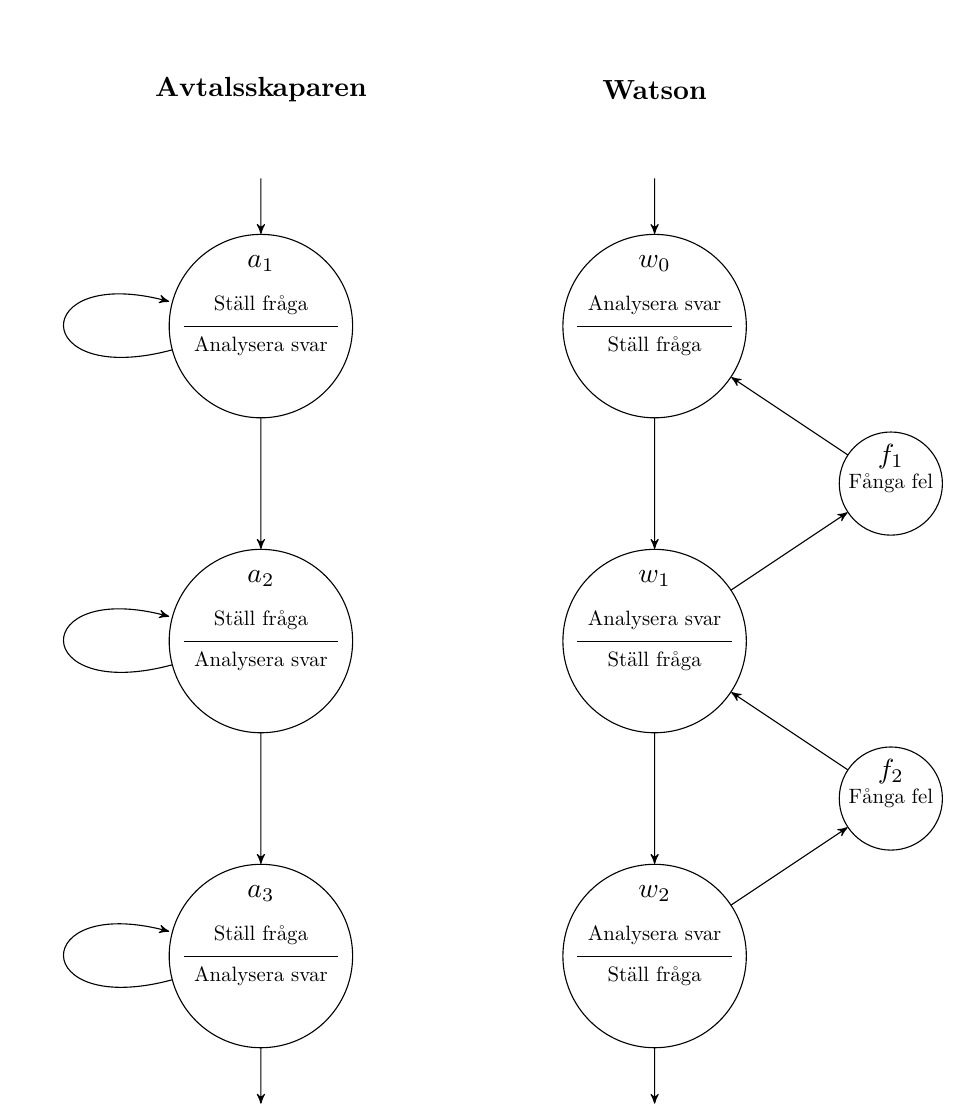
\begin{tikzpicture}[ring/.style={circle,draw=black,align=center,scale=0.75}]
        \node (SA) at (0, 3) [align=left] {\textbf{Avtalsskaparen}};
        \node (S0) at (0, 2) {};
        \node [label={[label distance=-0.6cm]90:$ a_1 $}] (S1) at (0,0) [ring] {Ställ fråga \\[-1ex] \rule{2.617cm}{0.4pt}\\ Analysera svar};
        \node [label={[label distance=-0.6cm]90:$ a_2 $}] (S2) at (0,-4) [ring] {Ställ fråga \\[-1ex] \rule{2.617cm}{0.4pt}\\ Analysera svar};
        \node [label={[label distance=-0.6cm]90:$ a_3 $}] (S3) at (0,-8) [ring] {Ställ fråga \\[-1ex] \rule{2.617cm}{0.4pt}\\ Analysera svar};
        \node (S4) at (0, -10) {};
        \draw[->] (S0) -- (S1);
        \draw[->] (S1) -- (S2);
        \draw[->] (S2) -- (S3);
        \draw[->] (S3) -- (S4);

        \draw[->] (S1) edge[loop left] (S1); 
        \draw[->] (S2) edge[loop left] (S2); 
        \draw[->] (S3) edge[loop left] (S3); 
        
        \node (WA) at (5, 3) [align=left] {\textbf{Watson}};
        \node (W0) at (5, 2) {};
        \node [label={[label distance=-0.6cm]90:$ w_0 $}] (W1) at (5,0) [ring] {Analysera svar \\[-1ex] \rule{2.617cm}{0.4pt}\\ Ställ fråga};
        \node [label={[label distance=-0.6cm]90:$ w_1 $}] (W2) at (5,-4) [ring] {Analysera svar \\[-1ex] \rule{2.617cm}{0.4pt}\\ Ställ fråga};
        \node [label={[label distance=-0.6cm]90:$ w_2 $}] (W3) at (5,-8) [ring] {Analysera svar \\[-1ex] \rule{2.617cm}{0.4pt}\\ Ställ fråga};
        \node [label={[label distance=-0.6cm]90:$ f_1 $}] (WC1) at (8,-2) [ring] {Fånga fel};
        \node [label={[label distance=-0.6cm]90:$ f_2 $}] (WC2) at (8,-6) [ring] {Fånga fel};
        \node (W4) at (5, -10) {};
        \draw[->] (W0) -- (W1);
        
        \draw[->] (W1) -- (W2);
        \draw[->] (W2) -- (WC1);
        \draw[->] (WC1) -- (W1);
        \draw[->] (W2) -- (W3);
        
        \draw[->] (W3) -- (WC2);
        \draw[->] (WC2) -- (W2);
        \draw[->] (W3) -- (W4);
        
        %\node (WF1) at (4, -1.5) {Accepterat};
        %\node (WF1) at (7, -1.5) {Felaktigt};
        
    \end{tikzpicture}
    \smallskip
    \caption{Skillnad i nodstruktur, mellan Watson och avtalsskaparen. Avtalsskaparen ställer en fråga och väntar på svar medan Watson läser ett svar och därefter ställer en fråga.}
    \label{fig:difference-watson-avtalsskapare}
\end{figure}

% Traversera avtalsskaparen
Eftersom avtalsmallen i avtalsskaparen endast består av frågor stannar systemet kvar i samma nod om svaret inte uppfyller nodens villkor. När systemet i figur~\ref{fig:difference-watson-avtalsskapare} går in i nod $a_1$ ställs den fråga som tillhör noden. Exempelvis kan denna fråga vara ``Hur många barn har du?'', och villkoret i noden är en siffra. Om användaren svarar med en färg, eller något annat som inte uppfyller villkoret kommer systemet stanna kvar i nod $a_1$. När användaren svarar med en siffra går systemet vidare till $a_2$.

% Traversera watson
Watson är mer generell än avtalsskaparen och vi var därför tvungna att ta fram lösningar för att den skulle passa vårt system. Som exempel kan noden $w_1$ representera samma fråga och villkor som $a_1$ (``Hur många barn har du?'', och ett nummer). Skillnaden mot avtalsskaparen är att frågan som är kopplad till $w_1$ sparas i noden $w_0$. Innan Watson går vidare till $w_1$ analyseras svaret som användaren ger till $w_0$ för att se om villkoret angivet i $w_1$ är uppfyllt.



% Felhantering watson
Om ett svar inte uppfyller villkoret går Watson till fångnoden $f_1$, för att därefter gå tillbaka till $w_0$ och ställa om frågan. Fångnoder är inte inbyggt i Watson utan är vanliga noder som skapas och anpassas av oss. Fångnoder har inga villkor som måste uppfyllas och behöver inte heller ge ett svar till $w_0$, utan går direkt till att ställa frågan. Alla frågor måste ha en fångnod för att ge användaren möjlighet att ange fel svar men ändå vara kvar i samma nod i dialogträdet. Utan en fångnod skulle Watson gå ur dialogträdet om användarens svar inte matchar ett villkor. För tabellen \mbox{Node} i databasen har varje fråga en referens till sin fångnod och denna sparas i kolumnen \mbox{\emph{catch\_node\_id}} för att kunna redigera och radera denna på Watson.

\FloatBarrier
\section{Avtalsskapare}
För administratörsverktyget så utgör avtalsskaparen den mest centrala delen. I det här avsnittet kommer vi beskriva dels den designprocess som föregick framtagandet av avtalsskaparen och hur avtalsskaparens dialogträd är visualiserad. 

\FloatBarrier
\subsection{Framtagande av avtalsskaparen} 
För att uppnå syftet med att förenkla för jurister att tillhandahålla avtal måste mallarna för dessa avtal skapas. En utmaning med administratörsverktyget var avtalsskaparen, alltså modulen där mallar för avtal skapas. Utmaningen i avtalsskapren grundar sig i att avtalsmallarna måste byggas på ett lagringsbart sätt och som vi enkelt kan översätta till IBM Watson. Enkelt i den bemärkelsen att genom avtalsskaparen abstraherar vi bort behovet att den som nyttjar avtalsskaparen behöver skriva dialoger i IBM Watson. Mer om hur vi integrerar avtalsskaparen med IBM Watson går att läsa under rubrik~\ref{subsec:integrate-watson}. 

Innan någon form av programmering för administratörsidan påbörjades var det viktigt att ta fram en ändamålsenlig design. Detta uppnådde vi genom en pappersprototyp som specificerade hur strukturen skulle se ut med tillhörande funktionalitet. I designen kom vi fram till ett antal viktiga koncept: En grafisk representation för relationen mellan frågorna inom en mall. Att de nödvändiga fälten för varje enskild fråga är: En frågetext, ett svar av en bestämd typ (till exempel ja,nej eller ett siffertal). Om det är en följdfråga krävdes även att ett villkor på föregående svar bestämdes. 

Ett exempel, en fråga kan vara ``har du barn'' det förväntade svaret specificeras till ``Ja'' eller ``Nej''. Därifrån kan följdfrågor bestämmas relaterade till svaret ``Ja'' respektive ``Nej''.

Fullständiga pappersprototypen finns tillgänglig i appendix~\ref{appen:papper_prototyp}
\subsection{Visualisering av avtalsmallar}
\label{sec:fragetrad:react}
%\newcommand{\sequence}{\textcolor{blue}{sekvens}}
%\newcommand{\choice}{\textcolor{red}{alternativ}}
%\newcommand{\node}{\textcolor{cadmiumgreen}{ruta}}
\newcommand{\sequence}{\mbox{Sequence}}
\newcommand{\choice}{\mbox{Choice}}
\newcommand{\node}{\mbox{Square}}

\newcommand{\tsquare}[1]{\tikz \draw[draw=#1, line width=1.5ex] (0,0) -- (1.5ex,0);}
\newcommand{\dinmamma}[2]{%
  \draw let
    \p1 = (#1.south),
    \p2 = (#2.north)
  in (#1.south) -- ($(#1.south)!0.5!(\x1,\y2)$) -| (#2.north);
}
\begin{figure}[htb]
    \centering
    \smallskip
    \hspace{70pt}% recenter it ungefärligt
    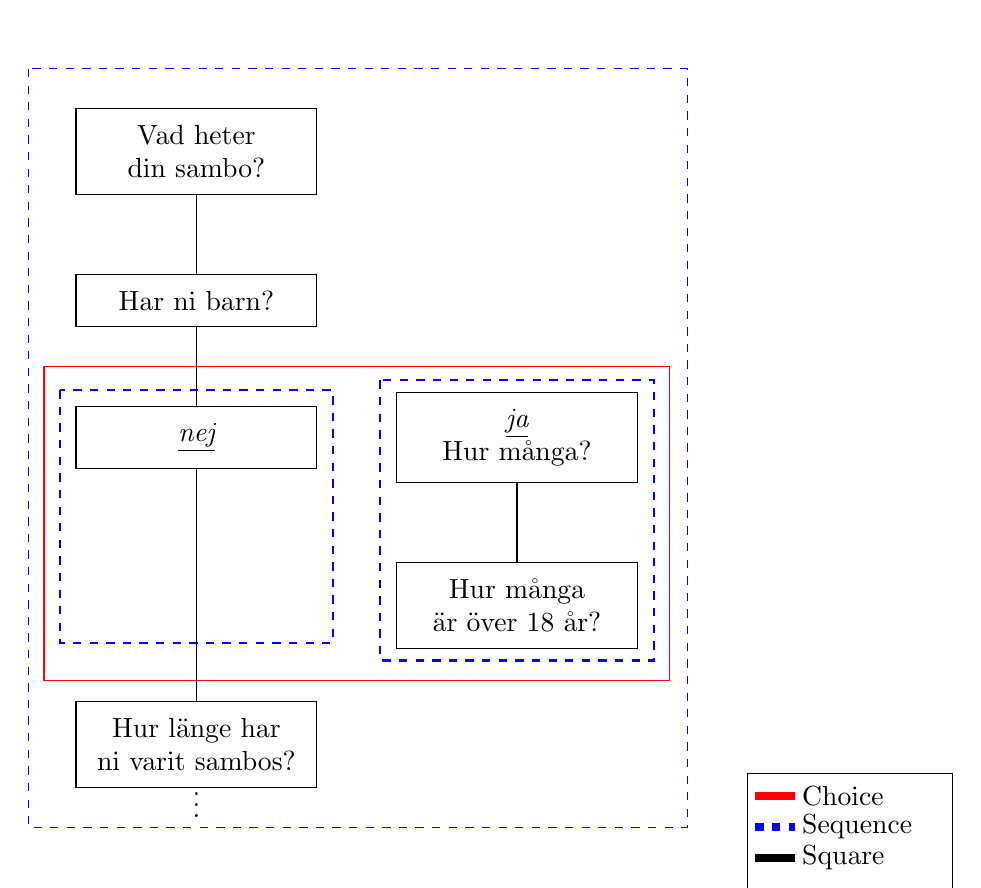
\begin{tikzpicture}[rekt/.style={rectangle,draw,inner sep=6pt,minimum width=50pt,text width=75pt,align=center}]
        \node (Q1) at (0, 0) [rekt] {Vad heter din sambo?};
        \node (Q2) [rekt, below=of Q1] {Har ni barn?};
        \node (Q21) [rekt,below=of Q2] {\textit{\underline{nej}}};
        \node (Q22) [rekt, right=of Q21] {\textit{\underline{ja}}\\Hur många?};
        \node (Q4) [rekt, below=of Q22] {Hur många är över 18 år?};
        \node (Q5) [rekt,draw=none,left=of Q4] {};
        \node (Q3) [rekt, below=of Q5] {Hur länge har ni varit sambos?};
        \node [node distance=-8pt,below=of Q3] {\vdots};
        
        %thick funkar inte??
        \draw[draw=blue,dashed] (Q1.north west) +(-0.6,0.5) rectangle ($(Q3.south east) + (4.7,-0.5)$);
        \draw[draw=red] (Q21.north west) +(-0.4,0.5) rectangle ($(Q4.south east) + (0.4,-0.4)$);
        \draw[draw=blue,dashed,thick] (Q21.north west) +(-0.2,0.2) rectangle ($(Q21.south east) + (0.2,-2.2)$);
        \draw[draw=blue,dashed,thick] (Q22.north west) +(-0.2,0.15) rectangle ($(Q4.south east) + (0.2,-0.15)$);
        
        \draw (Q1) -- (Q2) -- (Q21) -- (Q3);
        \draw (Q22) -- (Q4);
        \dinmamma{Q2}{Q22}
        \dinmamma{Q4}{Q3}
        
        \coordinate (legend) at (7,-8);
        \draw [fill=white] (legend) ++(0,0.1) rectangle +(2.6,-1.6);
        \draw [draw=red, line width=3pt] 
            (legend) ++(0.1, -1.2ex) -- ++(0.5, 0) node [label={[label distance=-0.7em]right:Choice}] {};
        \draw [draw=blue, dashed, line width=3pt]
            (legend) ++(0.1, -3.8ex) -- ++(0.5, 0) node [label={[label distance=-0.7em]right:Sequence}] {};
        \draw [draw=black, line width=3pt]
            (legend) ++(0.1, -6.4ex) -- ++(0.5, 0) node [label={[label distance=-0.7em]right:Square}] {};
    \end{tikzpicture}
    \smallskip
    \caption{Exempel på en avtalsmall. De röda och blå rutorna syns inte på webbsidan utan är hjälprutor för att visa den underliggande datastrukturen.}
    \label{fig:impl:html:tree}
\end{figure}
%Vårt dialogträd är en förenkling av IBM Watsons dialogträd som juristerna kan använda för att skapa sina kontrakt i.

Avtalsmallen är här en komponent i avtalsskaparen för att bestämma vilken ordning ett avtals frågor ska ställas i. Hur trädet kan se ut på webbsidan visas i figur~\ref{fig:impl:html:tree}. Varje nod innehåller vilken fråga som ska ställas och vilket sorts svar som accepteras, till exempel om bara ja eller nej accepteras.
%Anledningen till att det är ett träd och inte en lista med frågor är för att vissa frågor kan ha flera olika följdfrågor. Beroende på svaret användaren ger kan alltså olika följdfrågor ställas.
%Som exempel kan frågan ``hur många barn har du?'' ha vissa följdfrågor om man svarar att man har fler än kanske två barn och andra eller inga följdfrågor om man har två eller färre barn. 

En konversation med trädet i figur~\ref{fig:impl:html:tree} börjar med första frågan ``Vad heter din sambo?''. Efter att användaren har gett ett giltigt svar går trädet till nästa fråga som är ``Har ni barn?''. Om svaret inte är giltigt ställs frågan om tills ett giltigt svar har givits. Om användaren svarar ``nej'' går trädet vidare till ``Hur länge har ni varit sambos?'', men om användaren istället svarar ``ja'' kommer följdfrågorna ``Hur många?'' och ``Hur många är över 18?'' att ställas innan ``Hur länge har ni varit sambos?'' ställs.

\begin{minipage}{\textwidth}
Datastrukturen vi kom fram till för att representera en avtalsmall består av 3 delar:
\begin{itemize}
    \item\textbf{Square}\tsquare{black} är en ruta med en fråga som ska ställas och kriterium på giltiga svar till frågan.
    \item\textbf{Sequence}\tsquare{blue} är en vertikal lista som består av flera \node{} och/eller \choice{}. Frågorna i en \sequence{} kommer att ställas i ordning.
    \item\textbf{Choice}\tsquare{red} är en horisontell lista som består av minst två \sequence{}. Varje \sequence{} i \choice{} representerar olika vägar att fortsätta på beroende på svaret på föregående fråga.
\end{itemize}
\end{minipage}

Trädet i figur~\ref{fig:impl:html:tree} byggs upp genom att göra en \sequence{} på följande vis:
\par\makebox[\textwidth][c]{\ttfamily [\node(vad\ldots), \node(hur\ldots), \choice, \node(en\ldots), \ldots]}\par
där den första \node{} är frågan ``Vad heter din sambo?'', den andra ``Har ni barn?''. Det tredje elementet \choice{} består av en egen lista, nämligen:
\par\makebox[\textwidth][c]{\ttfamily [\sequence, \sequence]}\par
där den högra \sequence{} består av:
\par\makebox[\textwidth][c]{\ttfamily [\node(Hur många?), \node(Hur många är\ldots)]}\par
och den vänstra är uppbyggd på ett liknande vis.

Datastrukturen är designad för att enkelt rendera till HTML. Det blir enklare för att varje del i datastrukturen har en egen korresponderande React-komponent. Varje \node{} kan omvandlas till en \li{<div>} med specificerad bredd och höjd och alla \sequence{} och \choice{} omvandlas också till en varsin \li{<div>}. De två senare \mbox{\li{<div>}-arna} behöver endast rada upp sina barnelement åt ett visst håll och behöver inte modifiera storlek eller annat på barnen. Varje ruta i figur~\ref{fig:impl:html:tree} är alltså en React-komponent som alla är en \li{<div>}.


%Eriks original text nedan:
%Den här datastrukturen är designad för att förenkla renderingen till HTML. Det blir förenklat då varje del i datastrukturen har en egen naturlig korresponderande React-komponent. Varje \node{} kan omvandlas till en \li{<div>} med specificerad bredd och höjd. Alla \sequence{} och \choice{} omvandlas också till en varsin \li{<div>}, med skillnaden att de istället innehåller alla sina barn linjerade vertikalt nedåt respektive horisontellt åt höger. Varje ruta i figur~\ref{fig:impl:html:tree} är alltså en React-komponent som alla är en \li{<div>}.
\FloatBarrier

%\section{DEL x: Implementation av XYZ}\label{sec:delX}
%Mellan introduktion och avslutning finns ett eller sannolikt \emph{flera} avsnitt (``huvuddelen'') som innehåller själva bidraget eller implementationen.
%Ni får själva välja passande rubriker (INTE ``Huvuddel'' eller ``Bidrag'').  Rubrikerna i huvuddelen ska tillsammans med titeln ge en idé om vad som berättas, en ``berättelse''. (Exempel: ``Algoritm för automatisk igenkänning av stora fötter'', ``Design av databasen för användardata'', ``Optimering av minnesanvändning'', ``Implementation av djupinlärningssystemet'' etc.)

%Här kan ni beskriva implementationen, hur systemet används, etc.

%Beskriv gärna felhantering och riskanalys: vad kan gå fel när systemet kör/används, vad kan bli följden, och hur hanteras detta?

%\section{DEL x+1: Algoritm för igenkänning av stora fötter}
%Se avsnitt~\ref{sec:delX}.
%\section{DEL x+2: Optimering av minnesanvändning}
%Se avsnitt~\ref{sec:delX}.

\section{Krav och utvärderingsmetoder}\label{sec:krav}

%För de olika funktionaliteterna (och/eller motsv) i ert system, hur ska ni avgöra om de är tillräckligt bra utförda/implementerade? Var går gränsen för ``tillräckligt bra''? (Eller när är de ``för dåliga''?)

%Skilj på funktionalitet (vad ska systemet kunna göra) och krav (hur bra ska systemet vara). Själva funktionaliteterna har ni redan beskrivit i systemstrukturen eller huvuddelen nedan. (Har ni krav på saker ni beskriver först i huvuddelen kan ni lägga det här avsnittet efter huvuddelen.)

%Skriv tydliga krav \emph{som går att utvärdera}.  (Hur snabbt? Hur många användare? Hur strömsnålt? eller vad som är relevant).

%Beskriv hur utvärderingen ska gå till (automatiserade belastningstester, mätningar, en\-käter, fokusgrupper\ldots).
%Beskriv hur externa intressenter involveras i utvärderingen.

%För att säkerställa att systemet uppfyller det mål vi satt kommer vi utvärdera de olika delarna av systemet. Utvärderingen kommer använda olika metoder beroende på vilken roll delen har i systemet. De uppgifter systemets server har är annorlunda från chattgränssnittet på klientsidan och kan inte testas och utvärderas på sammas sätt.

Här förklaras vilka krav vi hade på systemet och hur vi testade att vi hade uppnåt dem.
Målen med projektet var att leverera en chattbott som underlättar avtalsfyllning samt en webbapplikation för jurister att skapa avtalsmallar i (se under rubrik~\ref{sec:syfte}).

\subsection{Krav}
%Det första kravet är att chattbotten ska rekommendera korrekt avtal hälften av fallen. 

%förslag Mats kommentar
Det första kravet är att chattbotten ska rekommendera korrekt avtal åtminstone hälften  av fallen av vårt test som finns i appendix~\ref{appen:recommendations}. Testfallen är framtagna så att hälften rätt är acceptabelt, då fallen har en varierande språknivå och de svåraste fallen är mycket ovanliga.

Det andra kravet är att administratörsverktyget ska vara användbar. För att kravet ska vara uppfyllt ska alla användare, med varierande teknisk kunskap, klara av att skapa avtalsmallar. Detta ska klaras av inom en rimlig tidsram, det ska inte ta användaren mer än fem minuter att skapa en mall. 

%Ett krav är att systemet ska identifiera användarens avsikt för att sedan, utifrån avsikten, bestämma vilket avtal som ska fyllas i. Det identifierade avtalets dialogträd ska sedan traverseras för att fylla i avtalet. När allt detta är slutfört ska all information som behövs för avtalet vara insamlad. 

%Vi har också kravet att om ett felaktig svar skrivs in ska frågan ska ställas igen.
%- Identifieringstestet anses lyckat då chattbotten föreslår rätt avtal majoriteten av försöken.
%- Avtalsskaparen är användarvänlig
%Testet anses lyckat när alla noder kan nås i rätt ordning och avtalet sparar alla svar när vi nått slutet.

\subsection{Utvärderingsmetoder}
Kravet på chattbotten testades genom att vi skrev manuellt i chattgränssnittet för att få rätt rekommendationer bland tre tillgängliga avtal: sambo-, kompanjon- och konsultavtal. Om vi i vår kommunikation med chattbotten hade en avsikt som matchade något av avtalen och chattbotten föreslog detta avtal blev det ett lyckat testfall. Vi gjorde detta åtta gånger för varje avtal och räknade antalet lyckade testfall. 

För att utvärdera det andra kravet avseende ett användarvänligt gränssnitt fick en testgrupp bestående av fyra personer (familj och bekanta) göra ett användartest. Den tekniska kunskapen hos personerna i testgruppen varierade, vilket är positivt då vi kan jämföra prestationen och förståelsen för systemet med hänsyn till deras kunskapsnivå. Användartestet utfördes genom att vi bad testpersonerna göra ett avtal medan vi observerade vad de gjorde. Testet gick ut på att de skulle återskapa avtalet i figur~\ref{fig:impl:html:tree} från grunden genom att lägga till frågor, och efter det bad vi testpersonen ta bort en fråga. Genom att utföra denna sekvens av instruktioner behöver användarna interagera med all funktionalitet på webbsidan. Under testet iakttog vi:
\begin{itemize}
    \item Vart de navigerade för att skapa en avtalsmall.
    \item Hur de försökte skapa en avtalsmall.
    \item Hur de försökte skapa frågor i avtalsmallen.
    \item Hur de försökte skapa förgreningar i avtalsmallen.
    \item Om de förstod hur en fråga togs bort.
\end{itemize}

%admin-verktyg
%På liknande sätt som beskrivs för användattesterna testas administratörsverktyget genom att en avtalsmall ska kunna skapas och sedan ska samma mall kunna traverseras genom dialog med chattbotten. Detta bekräftar att avtalet korrekt sparats till databasen, översatts till IBM Watson och återkopplats mot användargränssnittet.

%backend API
%För att testa hur servern tar emot API-anrop skrivs automatiserade tester som gör anrop till serverns samtliga API-funktioner. Kraven är att fel data får inte tas emot som argument och rätt data ska returneras som svar på specifika anrop. Därför jämförs HTTP-statuskoden~\cite{web:HTTP-status-codes} och datan i svaret med den statuskod och data som förväntas. 

%Databas
%Genom att testa samtliga API-anrop testas även indirekt systemets databas, eftersom samtliga API-anrop gör minst ett anrop till databasen. Då säkerställs att alla relationer mellan de olika tabellerna är korrekta, exempelvis att alla frågor som hör till ett kontrakt returneras när kontraktet begärs, och tas bort när kontraktet tas bort.

\section{Utvärderingsresultat}
%Beskriv resultaten av utvärderingen, när ni tillämpar de utvärderingsmetoder ni beskrivit i avsnitt~\ref{sec:krav}, och relatera utvärderingsresultaten till kraven i samma avsnitt.

%Skilj på utvärderingsmetoder och utvärderingsresultat, och mellan utvärderingsresultat (dvs resultat av användningen av utvärderingsmetoderna) och det större resultatet (nedan).

Resultatet från testet av rekommendationer av avtal var att systemet uppfyllde det första kravet vi ställde (se krav under avsnitt~\ref{sec:krav}). Systemet rekommenderade rätt avtal för åtminstone hälften av indatan som tagits fram, där varje indata hade en passande avsikt för ett visst avtal (se appendix~\ref{appen:recommendations} för alla testfall). Sammanlagt för varje exempelavtal var resultatet:
\begin{itemize}
    \item \textbf{samboavtal:} 50\%  
    \item \textbf{kompanjonsavtal:} 62.5\%  
    \item \textbf{konsultavtal:} 50\%
\end{itemize}

Den indata som användes för att testa rekommendationer utformades för att innehålla rätt avsikt, men med olika nivåer av klarhet. Vi förväntade oss att systemet skulle rekommendera samboavtal till indatan ''Jag vill flytta in med min flickvän'' men inte ''Har tjackat ny lya med kärringen''. Vi anser därför att testet är lyckat då systemet uppfyller kravet på åtminstone 50\% rätt.

Utvärderingen av användarvänligheten av administratörsverktyget gick dåligt, se avsnitt~\ref{sec:krav} för utvärderingsmetoden. Samtliga testpersoner förstod var de skulle navigera i verktyget för att skapa avtalsmallar och hur en avtalsmallen skapades. Det var dock inte uppenbart hur avtalsmallen namngavs eller att den kunde namnges. Att skapa frågor i mallen klarade alla testpersoner, däremot var hälften av testpersonerna förvirrade över var frågan skulle skrivas in, men efter letande hittade testpersonerna var detta kunde göras. 
Vidare var det oklart hur förgreningar skapades. En testperson uppgav att den fick chansa sig fram men chansade rätt på första försöket och en annan testperson skapade först fler följdfrågor istället för en förgrening, men lyckades också till slut. Samtliga testpersoner lyckades utan några förhinder med att ta bort en fråga. 



%Sammanfattningsvis anser vi att testet är lyckat, då samtliga testpersoner klarade av att fullborda den givna uppgiften. Det framgick dock att det inte var helt uppenbart hur förgreningar i avtalsmallen skapades och vart själva frågan skulle skrivas in.

%Mats kommentar 
Sammanfattningsvis anser vi att användbarhetstestens resultat var under förväntan och inte godtagbart. Ytterligare steg vidtogs och en ny design togs fram, dock hann vi inte genomföra ett nytt användbarhetstest. I den nya designen förbättrades hur avtalsnamn specificerades och var frågan skulle skrivas in genom att förbättra det grafiska gränssnittet och tydligare förklarande rubriker till dem olika fälten. 
%Lätt att skapa fråogr, däremot var förgreningar lite förvirrade, t ex la en testperson till fler följdfrågor istället för att förgrena och en annan uppgav att hen fick chansa sig fram
%


\section{Resultat och diskussion}
%Här beskriver ni först era resultat, vad ni åstadkommit.  Hur bra blev det?
%Sedan granskar ni era resultat kritiskt.  Varför blev det som det blev?  Var resultaten rimliga/bra/dåliga/o\-vän\-ta\-de\ldots?  
%Vad hade man kunnat göra annorlunda?  Hur relaterar era resultat till liknande arbeten?  

%\begin{itemize}
%\item Visa att utvärderingen är rimlig.
%\item Visa att utvärderingen, resultatet och analysen är vetenskapliga och ingenjörsmässiga.
%\end{itemize}

%Relatera till mål och syften etc i avsnitt~\ref{sec:syfte}.

Här tar vi upp resultaten av projektet och diskuterar det.  Resultatet innefattar webbsidan med avtalsskapare och chattgränssnittet, systemets server med tillhörande databas och slutligen en etikdiskussion. Överlag är vi nöjda med resultat då våra krav som ställdes på projektet uppfylldes.

\subsection{Webbsidan}
Webbsidans grundstruktur är klar men det är mycket funktionalitet som saknas än. Undersidorna kommer att tas upp i mer detalj här.

Avtalsskaparen färdigställdes inte. Administratörer kan skapa nya avtalsmallar och redigera existerande avtalsmallar. Mallarna renderas korrekt med noder på rätt ställen och linjer mellan dem. Frågor går att lägga till och frågor kan tas bort. Det går att lägga till flera följdfrågor till varje fråga och det går att specificera vilket villkor som krävs för att en viss följdfråga ska ställas (till exempel ja eller nej på föregående fråga).

%lägg till diskussion om kunskapsnivån och synen på denna ändrades i takt med att systemet utvecklades
En tidig målsättning för avtalsskaparen var att göra den så enkel som möjligt för att en jurist på egen hand ska kunna bygga en avtalsmall utom bakomliggande kunskap eller förståelse av IBM Watson. Skapande av avsikter och entiteter (som berördes i rubrik~\ref{subsec:IBM-watson-ass}) var dock mer krävande än så och för att skapa dessa krävs djupare kompetens i Watson. I rådande prototyp kan en administratör inte skapa egna avsikter och entiteter utan de är i nuläget fördefinerade. %Vidare diskussion under framtida arbeten? 

Chatten blev helt klar. Det går att skriva i textfältet för att skicka meddelanden till vår tjänst. 
 
\subsection{Serversidan}
I systemets databas representeras avtalsmallar på ett sätt som passar dialogträden i både IBM Watson Assistant och klientsidans avtalsskapare. Att kunna representera mallarna i båda dessa format~(se skillnader under~\ref{subsec:integrate-watson}) var målet med databasens design, och därför anser vi att resultatet av databasen är bra. 

I början av projektet gick en stor del av arbetet åt att komma fram med designen för databasen, eftersom det inte fanns direkt stöd i Watson för delar av den funktionalitet vi hade gett avtalsskaparen. Mycket tid lades alltså på att ta fram lösningar för kringgå Watsons begränsningar~(se~\ref{subsec:integrate-watson}). Trots dessa begränsningar gjordes bara en kompromiss, att frågor måste besvaras i kronologisk ordning. Om användaren anger mer information än vad frågan ber om sparas det inte, även om en följdfråga ber om den informationen.

Framtagningen av designen för databasen blev en flaskhals då utvecklingen av serverns API krävde en databas. Dock, tack vare den tiden vi lade på att göra en välgenomtänkt databasdesign fick vi en god uppfattning för hur resten av systemet på serversidan skulle struktureras. När designen av databasen var klar kunde modulerna till serverns API skrivas med relativ enkelhet. Vi hade inga prestandakrav på servern utan vi bedömmer resultatet av servern utifrån huruvida all behövlig funktionalitet är implementerad. All behövlig funktionalitet för avtalskapande existerar och därför anses resultatet av servern bra.
 
 %\paragraph{Användandet av React.js.}
 %Vi ansåg att användet av React var både nyttigt och utvecklande, vilket det har varit. Men att lära sig ett nytt ramverk som del av ett kandidatarbete visade sig vara mer tidskrävande än vad vi initialt förväntade oss. Ett exempel, vår administratörssida bygger mycket på nyttjande av olika formulär och inmatningsfält, något som vi upplevde som omständigt och som vi upptäckte i våra efterforskningar vi inte är ensamma om att tycka. %https://reactjsexample.com/build-forms-in-react-without-the-tears/
%En viktigt lärdom att ta med sig från det här, är att det är viktigt att göra efterforskningar innan ett projekts påbörjande avseende  till exempel ramverket. För att  så sätt utifrån en lämplighetsbedömning avgöra vad vi borde använda.

\subsection{Etik}
Vårt system kommunicerar via textdialog med användaren, vilket leder till att individer med vissa funktionsnedsättningar blir begränsade i användningen av vårt system. Exempelvis kan blinda individer inte använda vårt system alls, då de inte kan läsa vad systemet svarar. Detta kan lösas genom att lägga till stöd för text-till-tal och tal-till-text för att kunna prata med systemet istället~\cite{web:srf-IT}. Ett annat exempel på exkluderade av individer är de som har dyslexi då systemet kan ha svårt att förstå vad individen försöker yttra om det är många eller grova stavfel i texten.

%Det är svårt att göra vår tjänst lättillgänglig för alla. Det går inte att anpassa systemet till alla individer samtidigt. Kunderna som köper och erbjuder vårt system måste ha detta i åtanke för att antingen vidareutveckla systemet för att bli mer anpassat eller skapa alternativ till individer med någon begränsning.

Vårt system bidrar till att den digitala klyftan växer. Den digitala klyftan är ett begrepp som beskriver hur lösningar blir mer och mer tekniska medan vissa i samhället inte hänger med i utvecklingen~\cite{web:digitala_klyftan}. Systemet bidrar till klyftan genom att vi har gjort en teknisk lösning av avtalsifyllning som annars i många fall har skett i fysisk form med en jurist. Om juristbyråer helt skulle övergå till vårt system skulle individer som är tekniskbegränsade få problem att få hjälp med den här sortens problem.

%\{snacka om det är okej att samla in data\}
Vårt system samlar enbart in den information som en jurist explicit uppger krävs för att avtalet ska kunna tecknas. Informationen som lagras är enbart tänkt att användas i avtalen och inte till något annat. Det är alltså ingenting som säljs vidare eller lämnas ut till någon ytterligare part. Givet detta har inga särskilda åtgärder vidtagits för att garantera informationsäkerhet genom till exempel inloggningsystem eller kryptering av data. Eftersom vårt system med stor sannolikhet kommer behandla känslig data som personnummer och bankkontonummer bör denna data skyddas. Detta för att ingjuta tillit hos användaren att datan inte kommer hamna i fel händer.

\subsection{Resultat gentemot relaterade system}
%hur relaterar era result till relaterade arbeten
Skillnaden gentemot de liknande systemen (se rubrik~\ref{subsec:similair-sys}) och vårt system kommer främst beskrivas utifrån användareperspektivet av chattgränssnittet. Anledningen till att vi inte berör de liknande systemens motsvarighet till avtalsskaparen är för att de flesta är betaltjänster som vi inte har tillgång till inom ramen för det här projektet. 
%tolka avsikt och välja 
Genom vårt system kringgår vi problematiken med att en användare inte är insatt i vad det korrekta namnet är för ett specifikt avtal är. Givet ett exempel i talspråk ``att sälja en sak'' är ``överlåtelse av egendom'' i juridiska termer, och då går vi inte in på att det även en är skillnad på lös och fast egendom. Sammanfattningvis finns det många termer som inte är uppenbara för någon som inte är påläst~\cite{web:consector}. Att vårt system erbjuder möjligheten att tolka en avsikt kontra de liknande system där en användare explicit måste, med knappval, välja det avtal den vill teckna är en markant skillnad, då de i vårt system får hjälp av hitta rätt avtal. För en användare som är insatt och vet vad den vill, till exempel teckna ett samboavtal, blir det också enklare. I de liknande systemen måste rätt avtal hittas och klickas på medan i vårt system så kan användaren direkt skriva `Jag vill teckna ett samboavtal''. 

%Genom dessa fördelar, hjälp av ta fram rätt avtal och snabbåtgång till avtal, har vårt system ett potential kunna erbjuda bättre stöd och effektivare hantering för användaren.

%smartare hjälp och sätt att fylla i avtalen? 


%Begränsningar och tillkorta kommande/problem? 
En begränsning för systemet är Watsons kapacitet. Om en användare använder för otydliga, grammatiskt inkorrekta eller felstavade ord kommer det leda till att Watson inte kan hjälpa till och systemet sannolikt stannar i ett. Likväl såsom våra test visar förstår inte Watson i nuläget inte alltid grammatiskt korrekta meningar, vilket är ett tillkortakommande med grund i att Watson behöver tränas upp mer för att få en bredare kunskap och förståelse.  


\section{Slutsatser}
%Här sammanfattar ni och upprepar ert bidrag (resultaten av ert projekt) och förklarar dess vikt och användning. 
Projektet resulterade i ett chatt\-gränss\-nitt och ett administratörsverktyg. Chattgräns\-snittet kommunicerar med chattbotten för att identifiera vad för avtal kunden behöver och hjälper sedan till att fylla i det. För att göra avtal tillgängliga för chattbotten skapas mallar för avtalen i adminstratörsverktyget. Detta sker helt utan att administratören har kunskap om hur det bakomliggande systemet, IBM Watson, fungerar. 

%Vad var viktigt/nytt/intressant?  (INTE i termer av vad ni lärde er, utan för den som läser rapporten, funderar på att göra ett liknande system, vidareutveckla ert system, etc.)

% Efter projektets designfas kunde datarepresentationen användas för att ta fram databasdesignen och adminstratörsverktyget. 

Vi har alltså förenklat för jurister att skapa specifika avtalsmallar i IBM Watson. Att skapa den här förenklingen har styrt hela projektet. En datarepresentation av en avtalsmall togs fram som både är intuitiv för användaren och kompatibel med IBM Watson. Skulle en vidareutveckling på detta projekt ske är den underliggande designidén en bra grund att utgå i från. 

%har vi nåt mer nytt/intressant?

\section{Framtida arbeten}

%- icke-kronologisk ordning
Dialogträden med kontrakten och tillhörande frågor är fullt fungerande i nuvarande form. Frågorna ställs i turordning, när en fråga besvaras på ett sätt som uppfyller villkoret går systemet vidare till nästa fråga och upprepar processen . Det finns dock en svaghet i implementation, frågor måste besvaras i kronologisk ordning. 

Exempelvis kan användaren ange ''Hej! Jag heter Arne Björk och jag ska flytta in med min flickvän på Gatuvägen 3 den 6 juni'' till chattbotten. Systemet kommer då identifiera att användarens avsikt är att flytta in med en partner, och rekommendera att användaren tecknar ett samboavtal. 

Däremot kommer resten av informationen, namnet och datumet, inte sparas, även om det är ett relevant svar på en senare fråga. För att komma runt detta bör svarets samtliga avsikter och entiteter analyseras för att kunna avgöra om det är information som kan användas senare.

%- säkerhet
Skulle systemet lanseras publikt skulle det även vara tvunget att följa de regler som anges av dataskyddsförordningen (GDPR)~\cite{web:gdpr}. Därför är ett annat framtida arbete att implementera inloggningsfunktioner i systemet. Det skulle möjliggöra underskrift av avtal eftersom användaren då kan styrka sin identitet. Dessutom, I den nuvarande versionen av systemet kan vem som helst skapa, redigera och ta bort samtliga avtalsmallar och tillhörande frågor. För att undvika detta bör systemet säkerställa att endast användare med rätt behörighet kan göra anrop till serverns API. En lösning till detta problem är att implementera JSON Web Tokens som ger varje användare en unik nyckel när de loggar in som skickas med varje anrop för att verifiera behörighet~\cite{web:jwt}.
%- responsiv/design - så som drag-and-drop och css som inte är spartansk
%- visa ifyllda avtal

Funktionalitet för att redigera avtalsmallar, som i att flytta på noder med ``drag and drop'', är något som inte blev implementerat i avtalsskparen. Om denna funktionalitet implementerades skulle redigering av existerande avtal underlättas.

Datastrukturen för avtalsmallen på klientsidan som beskrivs under rubrik~\ref{sec:fragetrad:react} kan bli effektivare. För hitta en nod (Choice, Sequence eller Square) i trädet, för att till exempel redigera, måste alla noder sökas igenom då de inte är organiserade på något sätt. Eftersom avtalen, och därmed träden, är relativt små märks inte detta av tidsmässigt. Men det är fortfarande onödigt många beräkningar som körs och det kan potentiellt bli för långsamt i framtiden.

%pdfer
I en slutgiltig version av systemet så kommer vi även vilja att både skapade och ifyllda avtalsmallar ska kunna granskas av administratör respektive användare. De svar som användaren har angett ska sparas och presenteras på ett tydligt sätt, i olika format beroende på situationen. När administratören granskar dokument kan det ske direkt på webbsidan medan användaren kan få en .pdf-fil för att spara sina svar.

%\{dessa delar måste ses över och passar eventuellt bättre in på avgränsningar\}
%- villkorsskaparen, att de facto kunna skapa egna avsikter och entiter och kunna editera dessa 

%\section{Framtida arbete}
%Här beskriver ni potentiella framtida utvecklingar av systemet. Var finns förbättrings\-poten\-tial och vad kan man bygga vidare på? Vilka intressanta utvidgningar hann ni inte med?

%Observera att risk\-be\-döm\-ning, tids\-planering, relation till kursmål \emph{inte} hör hemma i slutrapporten.

% Use one of these:
%   IEEEtranS gives numbered references like [42] sorted by author,
%   IEEEtranSA gives ``alpha''-style references like [Lam81] (also sorted by author)
\bibliographystyle{IEEEtranS}
%\bibliographystyle{IEEEtranSA}

% Here comes the bibliography/references.
% För att göra inställningar för IEEEtranS/SA kan man använda ett speciellt bibtex-entry @IEEEtranBSTCTL,
% se IEEEtran/bibtex/IEEEtran_bst_HOWTO.pdf, avsnitt VII, eller sista biten av IEEEtran/bibtex/IEEEexample.bib.
\newpage
\bibliography{bibconfig,refs}
%\bibliography{refs}

\newpage
\appendix %%%% markerar att resten är appendixar

\section{Rekommendationstest} \label{appen:recommendations}

Följande termer matades in manuellt i chattbotten för att se om det matchar mot rätt avtal. De tre avtalen som fanns var samboavtal, kompanjonsavtal och konsultavtal.

Resultatet från försök att matcha mot samboavtal:

\begin{tabularx}{\textwidth}{ |X|l| } \hline
\textbf{Indata} & \textbf{Matchade}  \\ \hline
Jag vill flytta in med min flickvän & Ja \\ \hline
Min pojkvän och jag ska flytta ihop & Ja \\ \hline
Jag och min partner ska köpa lägenhet & Ja \\ \hline
Nästa vecka ska jag flytta in hos min respektive & Nej \\ \hline
Min kille kommer flytta in här nästa vecka & Ja \\ \hline
Tjejen flyttar in & Nej \\ \hline
Gumman och jag ska flytta ihop  & Nej \\ \hline
Har tjackat ny lya med kärringen  & Nej \\ \hline
\end{tabularx}

Resultatet från försök att matcha mot kompanjonsavtal:

\begin{tabularx}{\textwidth}{ |X|l| } \hline
\textbf{Indata} & \textbf{Matchade}  \\ \hline
Jag ska starta nytt företag med en kollega & Ja \\ \hline
Jag ska starta nytt med en partner & Ja \\ \hline
Jag och Gurra ska starta ny firma & Nej \\ \hline
Har startat firma med en gammal kollega & Ja \\ \hline
Öppnade ny affär med en kompis & Ja \\ \hline
Har slått ihop min firma med en ny partners firma & Ja \\ \hline
Kommer starta nytt med min gymnasieklasskompis & Nej \\ \hline
Har startat bilmek med kumpan & Nej \\ \hline
\end{tabularx}

Resultatet från försök att matcha mot konsultavtal:

\begin{tabularx}{\textwidth}{ |X|l| } \hline
\textbf{Indata} & \textbf{Matchade}  \\ \hline
Jag har anställt en konsult & Ja \\ \hline
Jag har blivit anställt som konsult & Ja \\ \hline
Vi ska ta in en konsult & Nej \\ \hline
En firma kontaktade mig om en konsulttjänst & Nej \\ \hline
Vi ska hyra in en rådgivare & Nej \\ \hline
Jag erbjöd rådgivning & Nej \\ \hline
Vi tog in en expert & Ja \\ \hline
Firman anlitade en konsult & Ja \\ \hline
\end{tabularx}



\newpage
\section{Designprototyp} \label{appen:papper_prototyp}
\FloatBarrier
I figur~\ref{fig:design_frontend_1} följer den designprototyp som togs fram för avtalsskaparen. I en första prototyp vägde en funktionell layout tyngre än en snyggare grafisk design. Detta är även en design som innehåller viss funktionalitet som inte implementerats i nuvarande version, men som beskrivs under framtida arbeten. 

%\begin{figure}[h]
%    \smallskip
%    \begin{subfigure}[t]{0.49\textwidth}
%        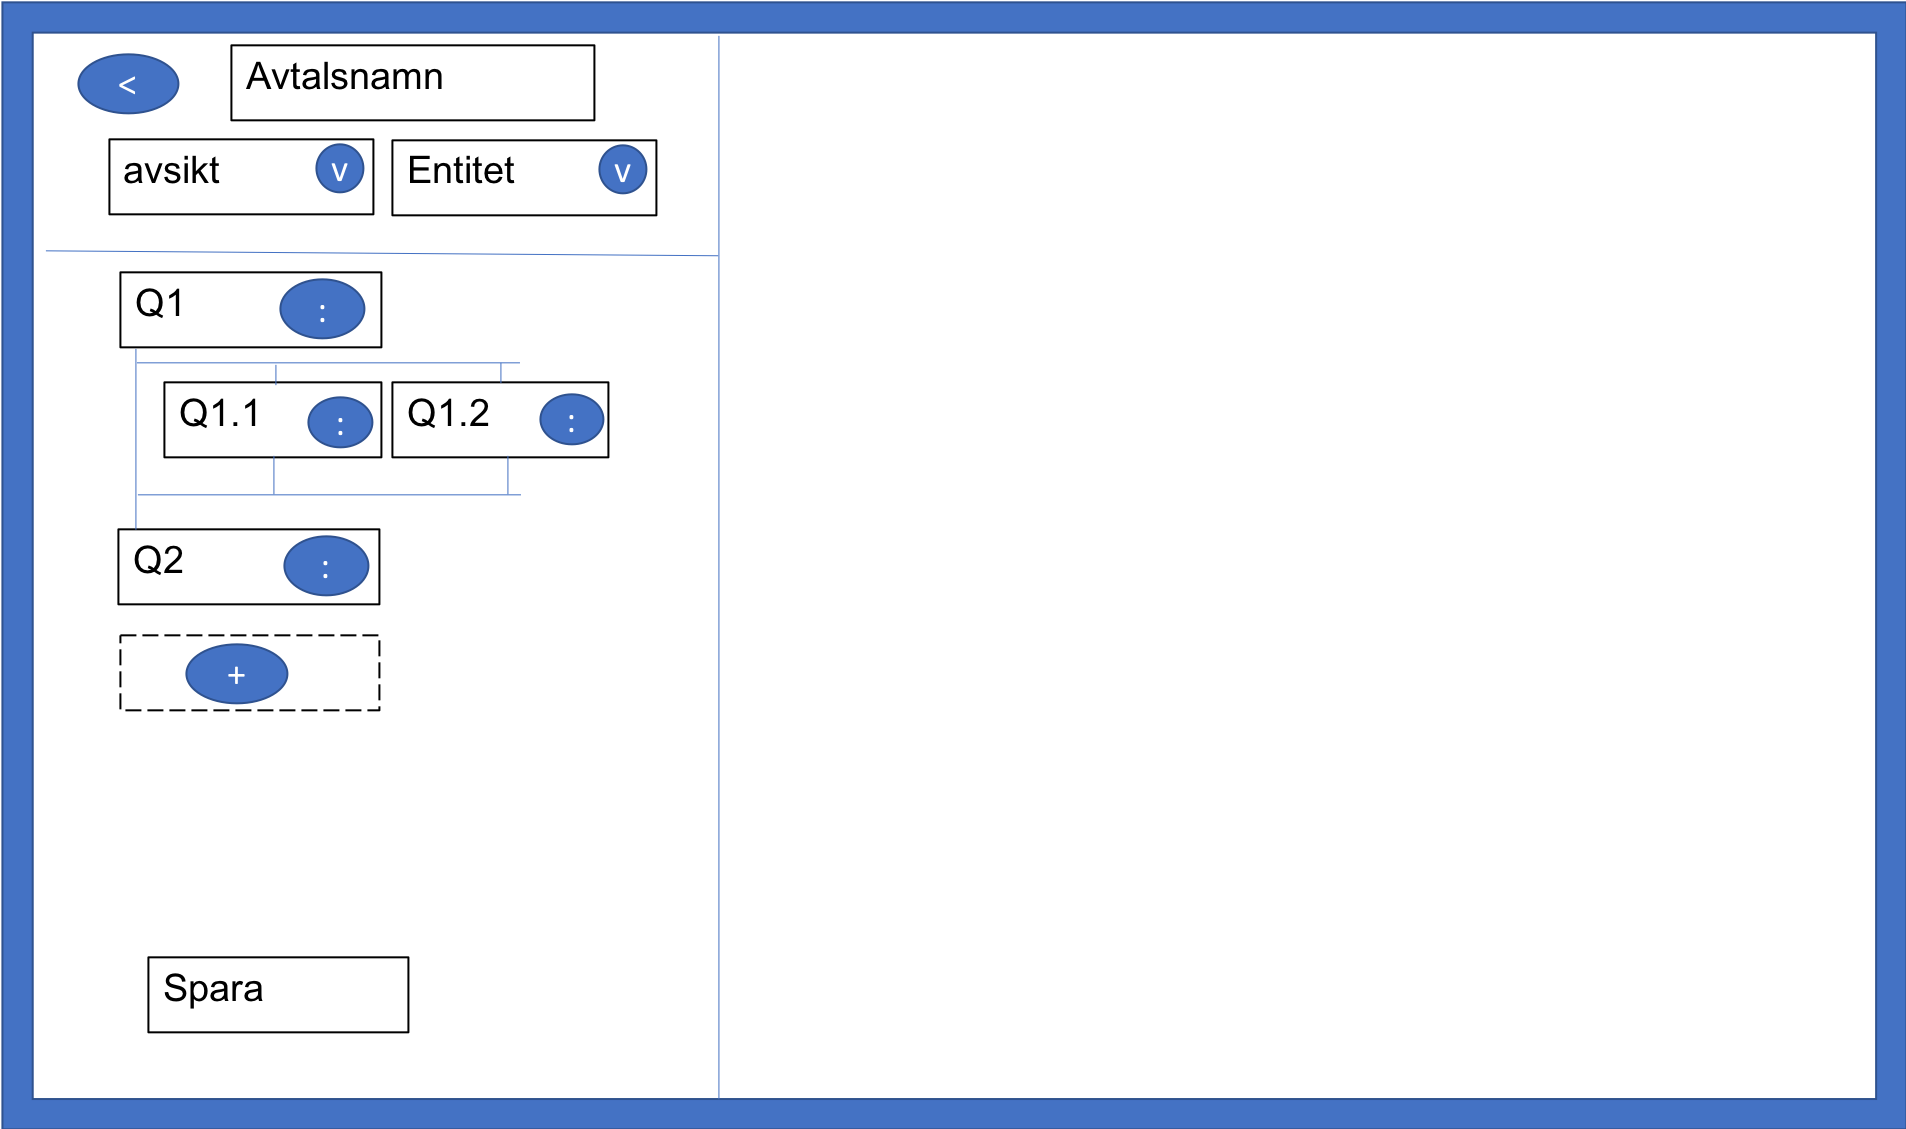
\includegraphics[width=\linewidth]{img/avtalsskapare_1.png}
%        \caption{Initial vy för avtalsskaparen med ett exempel dialogträd för en avtalsmall}
%    \end{subfigure}\hfill%
%    \begin{subfigure}[t]{0.49\textwidth}
%        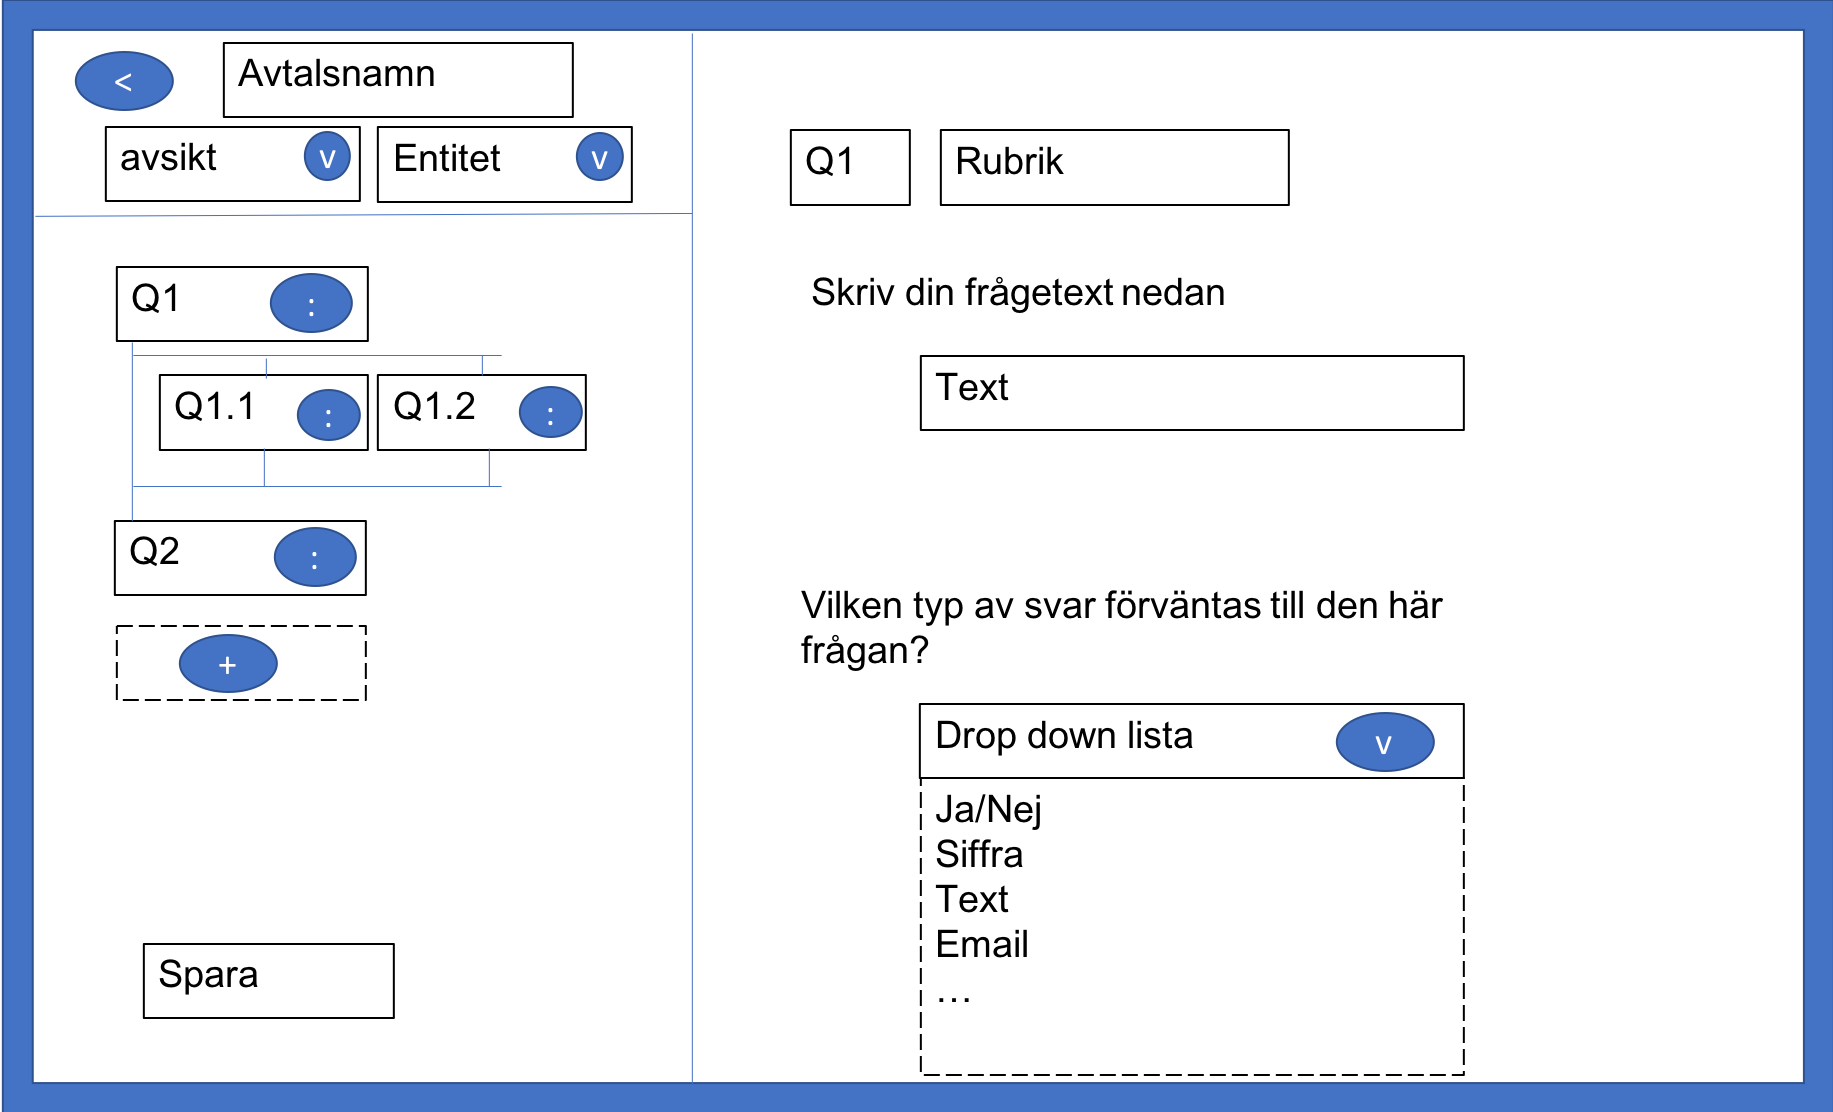
\includegraphics[width=\linewidth]{img/avtalsskapare_2.png}
%        \caption{Fönster som kommer fram när en av noderna i dialogträdet klickas på}
%    \end{subfigure}
%    
%    \vspace{1cm}
%    \begin{subfigure}[t]{0.49\textwidth}
%        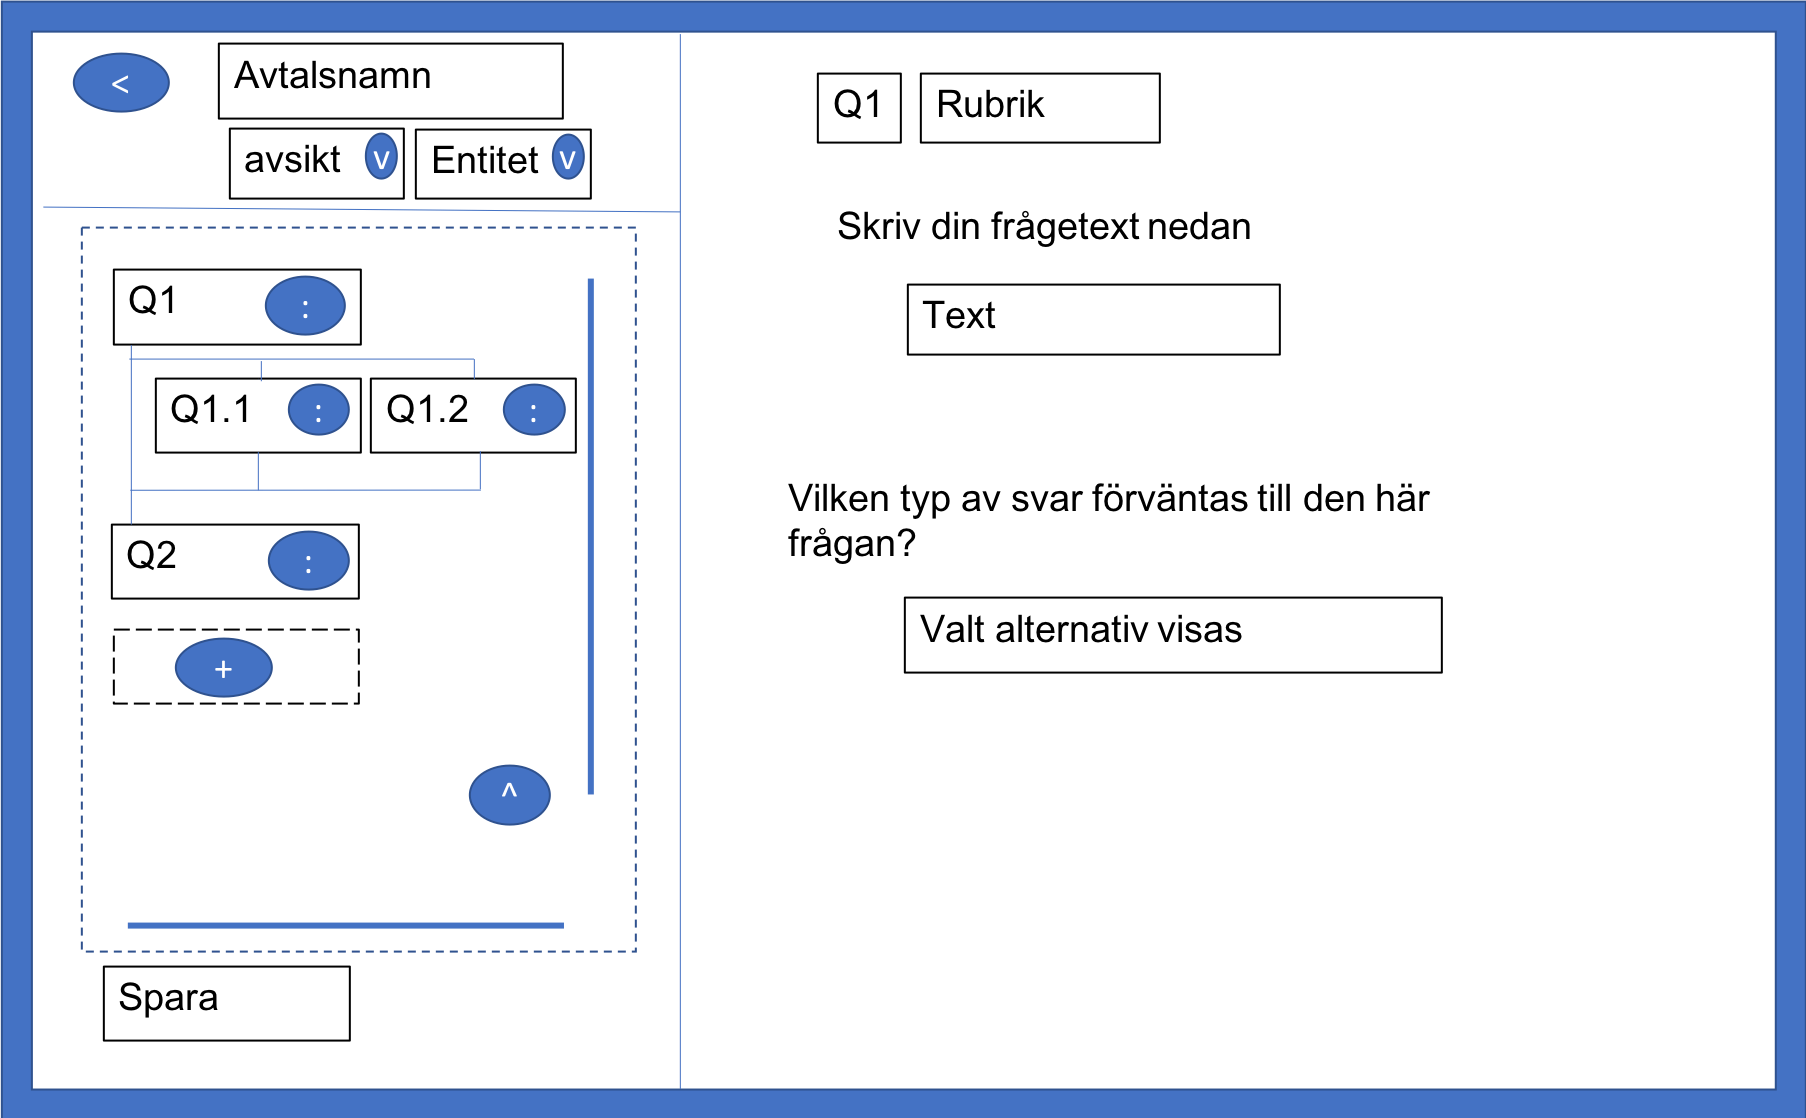
\includegraphics[width=\linewidth]{img/avtalsskapare_3.png}
%        \caption{Efter att typ av förväntat svar för den här frågan har valts så visas det valda alternativet}
%    \end{subfigure}\hfill%
%    \begin{subfigure}[t]{0.49\textwidth}
%        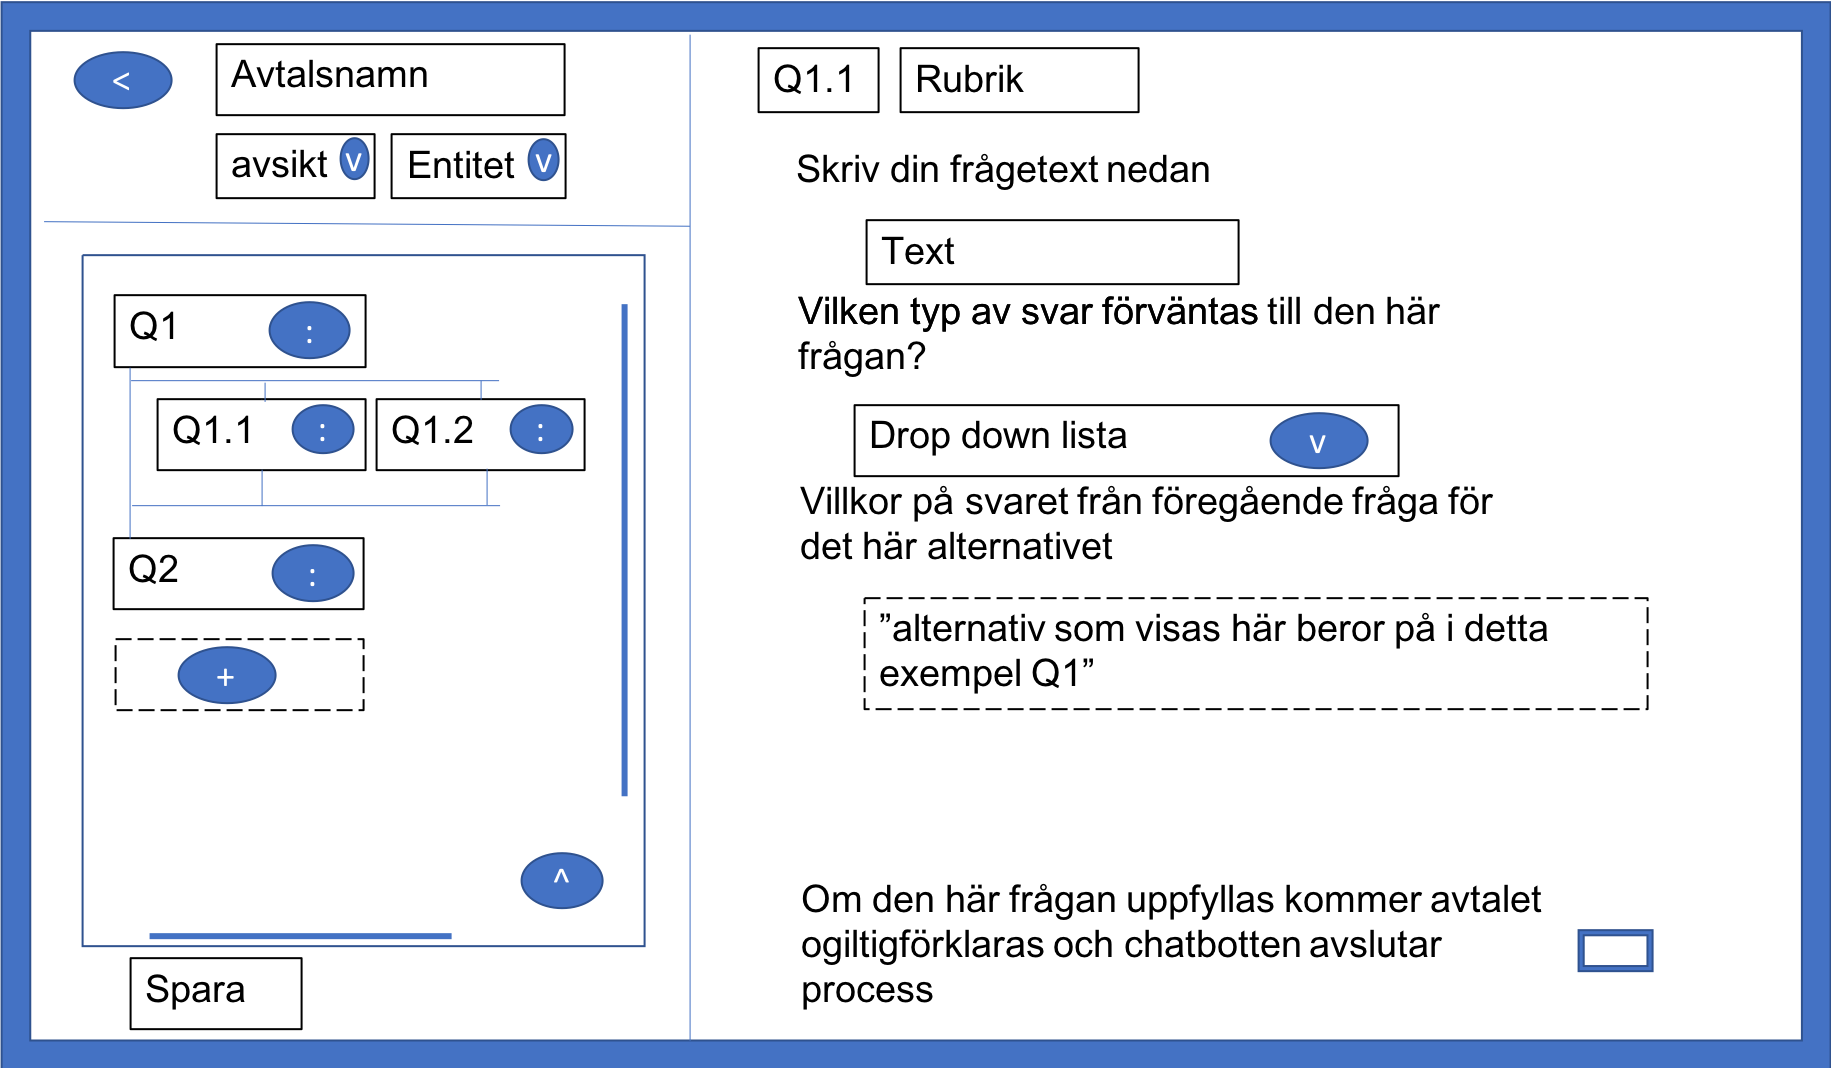
\includegraphics[width=\linewidth]{img/avtalsskapare_4.png}
%        \caption{Vi är nu i en följdfråga, tillkommet till denna vy är att en administratör måste definiera vilket %svarsalternativ från föregående fråga som leder till den här frågan, även möjligheten att avsluta processen om svaret på %en följdfråga skulle leda till det.}
%    \end{subfigure}
%    \smallskip
%    \caption{Pappersprototypen för avtalsskaparen.}
%    \label{fig:appendix:paper:prototype:of:avtalsskaparen}    
%\end{figure}

\begin{figure}[H]
    \ContinuedFloat*
    \centering
    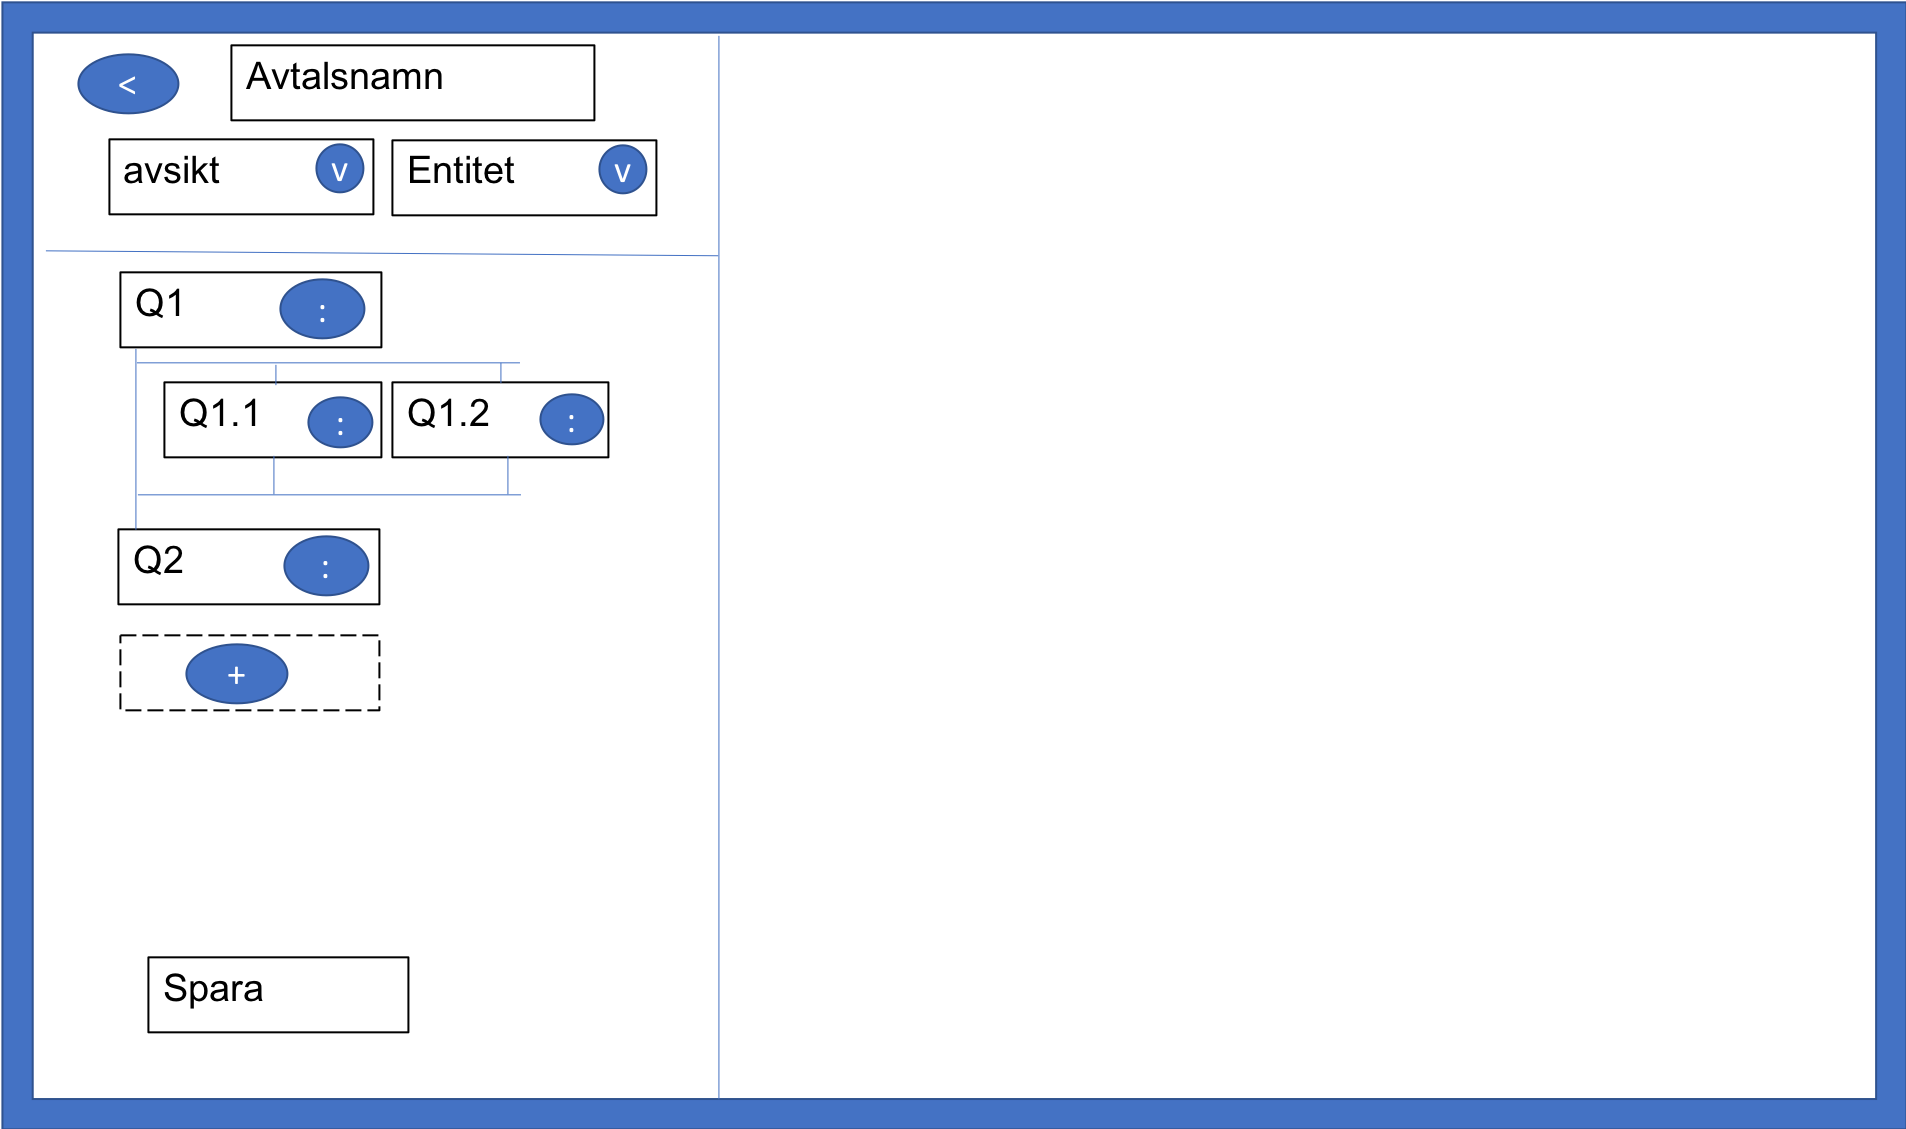
\includegraphics[width=0.8\linewidth]{img/avtalsskapare_1.png}
    \caption{Initial vy för avtalsskaparen med ett exempel dialogträd för en avtalsmall}
    \label{fig:design_frontend_1}
\end{figure}

\begin{figure}[H]
    \ContinuedFloat
    \centering
    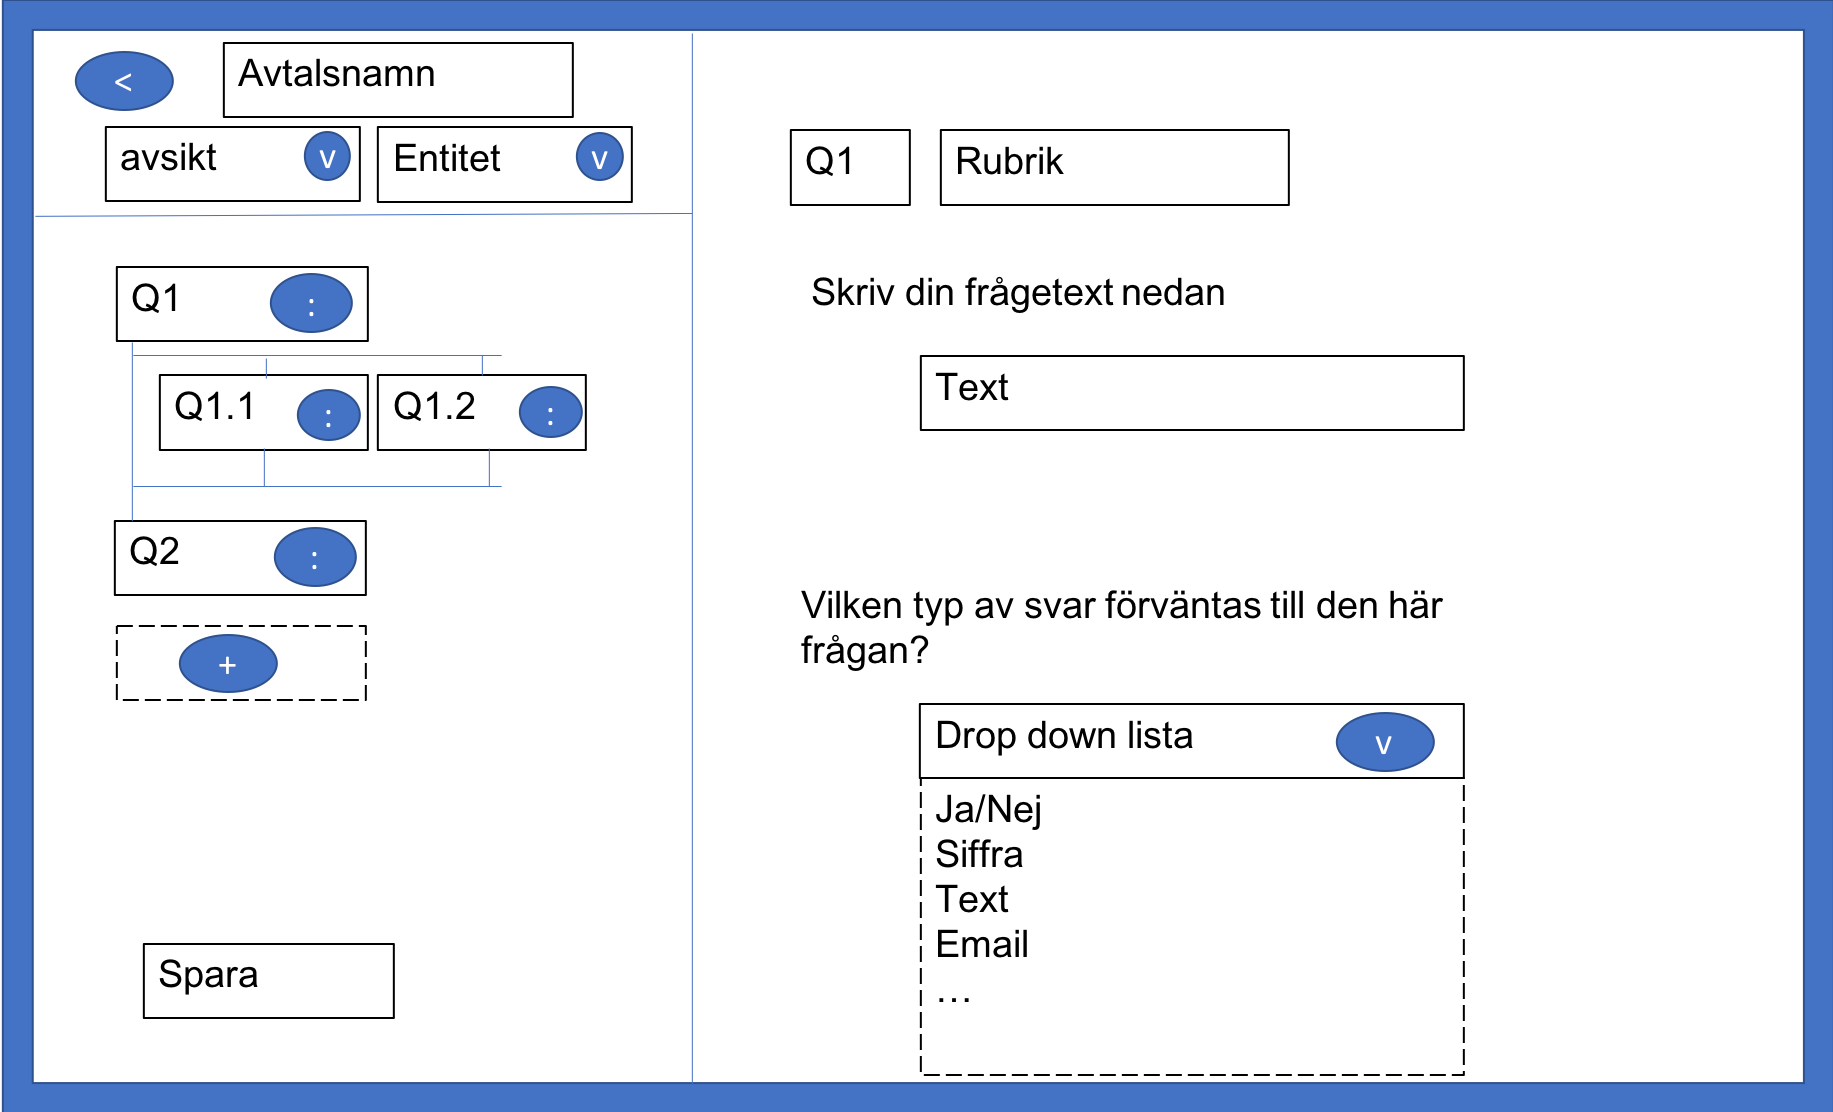
\includegraphics[width=0.8\linewidth]{img/avtalsskapare_2.png}
    \caption{Fönster som kommer fram när en av noderna i dialogträdet klickas på}
    %\label{fig:design_frontend_2}
\end{figure}

\begin{figure}[H]
    \ContinuedFloat
    \centering
    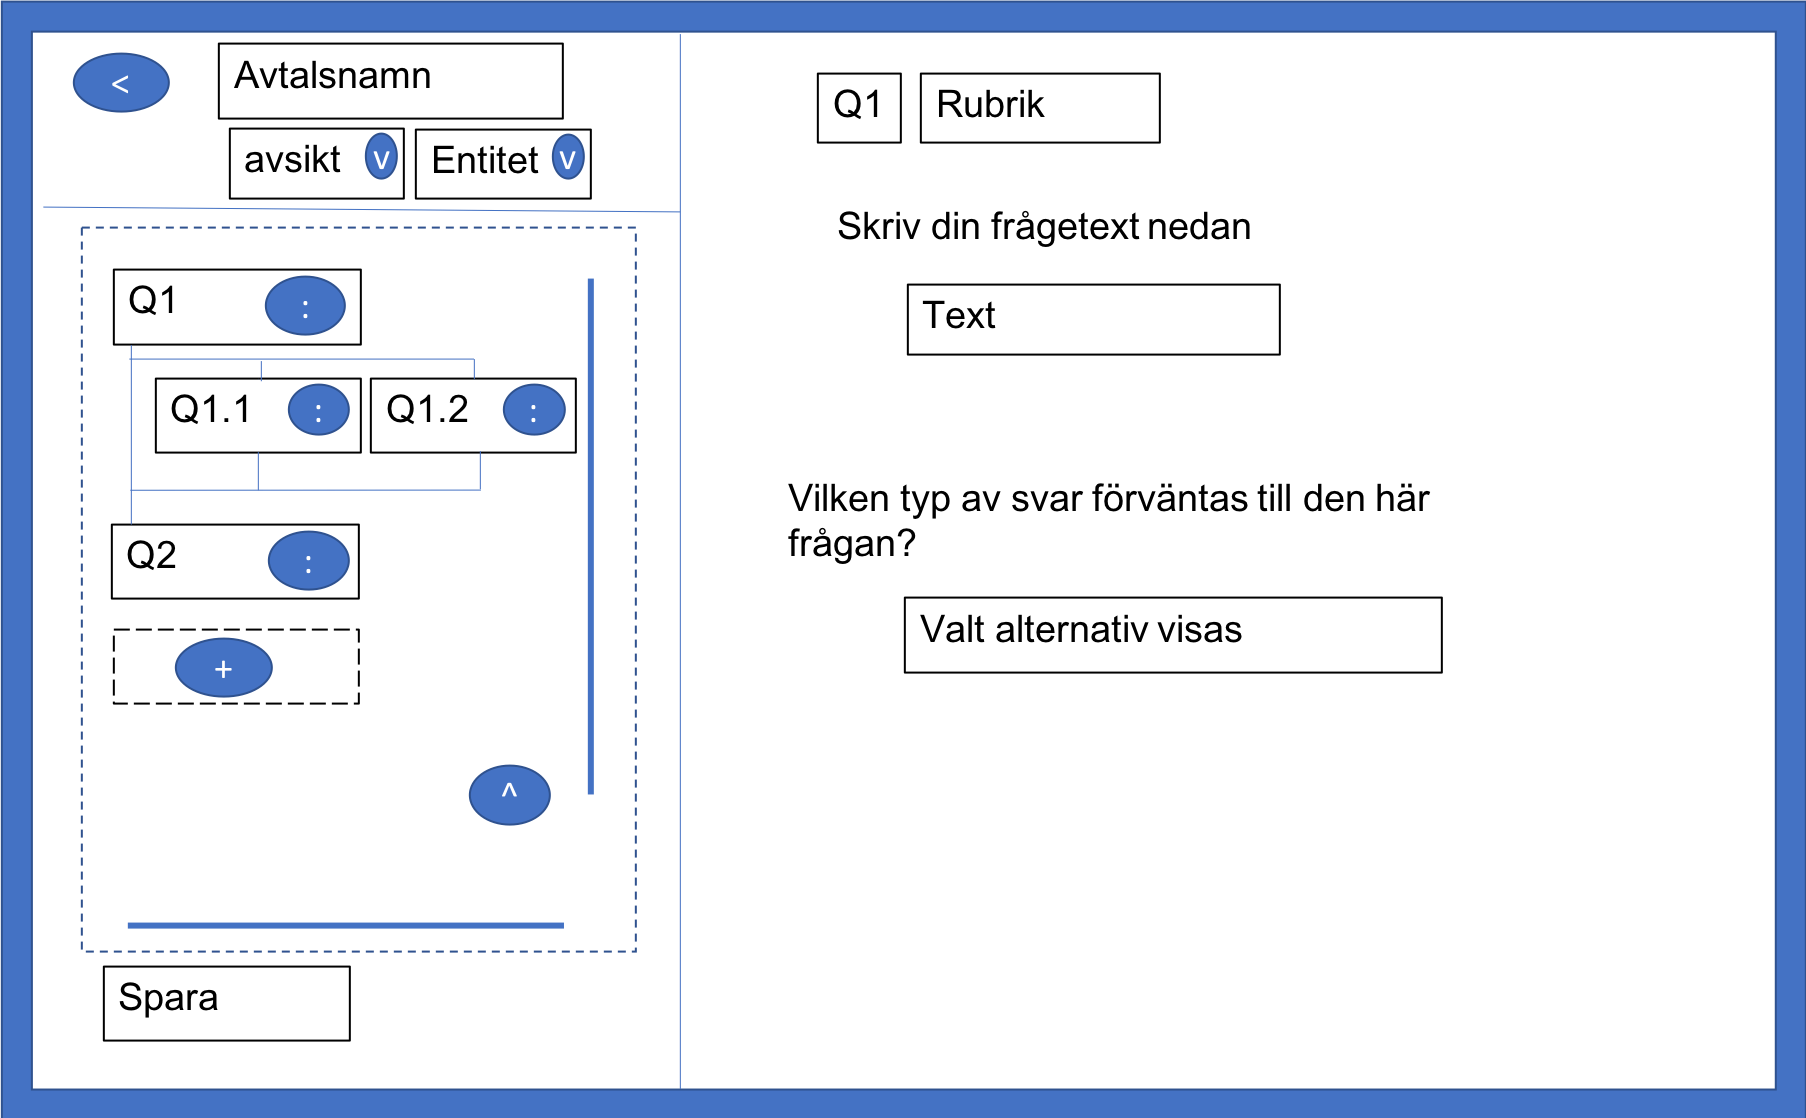
\includegraphics[width=0.8\linewidth]{img/avtalsskapare_3.png}
    \caption{Efter att typ av förväntat svar för den här frågan har valts så visas det valda alternativet}
    %\label{fig:design_frontend_3}
\end{figure}

\begin{figure}[H]
    \ContinuedFloat
    \centering
    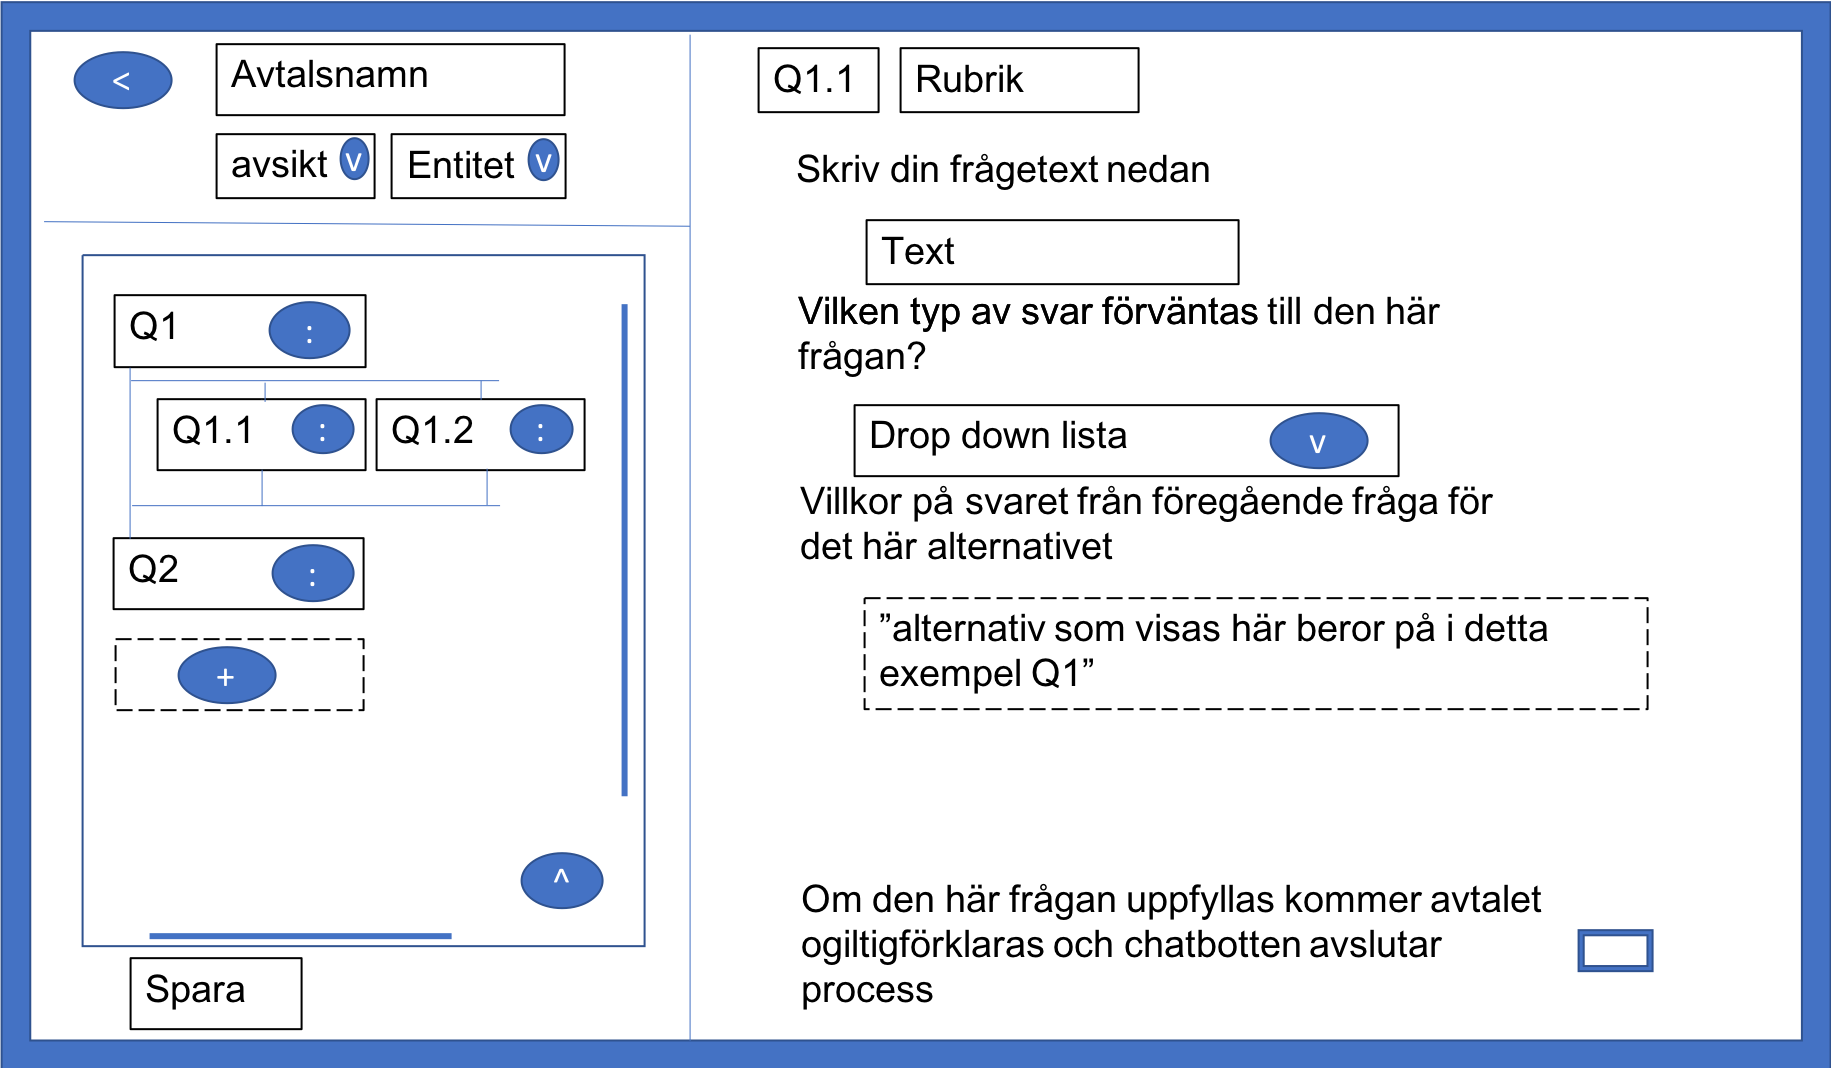
\includegraphics[width=0.8\linewidth]{img/avtalsskapare_4.png}
    \caption{Vi är nu i en följdfråga, tillkommet till denna vy är att en administratör måste definiera vilket svarsalternativ från föregående fråga som leder till den här frågan, även möjligheten att avsluta processen om svaret på en följdfråga skulle leda till det.}
    %\label{fig:design_frontend_4}
\end{figure}
%\section{Gruppregler}
%\begin{itemize}
%    \item Arbete på polacksbacken, vardagar 10-15 om inget annat är sagt.
%    \item Arbete när det är arbete, paus när det är paus.
%    \item Alla beslut ska tas demokratiskt och för mycket tid ska inte läggas onödig diskussion.
%    \item Fikaansvarig ska ta med fika minst en gång under sin mandatsperiod. Rollen byts varje vecka.
%\end{itemize}

%\section{Tidsplan}

%\begin{figure}[H]
%    \centering
%    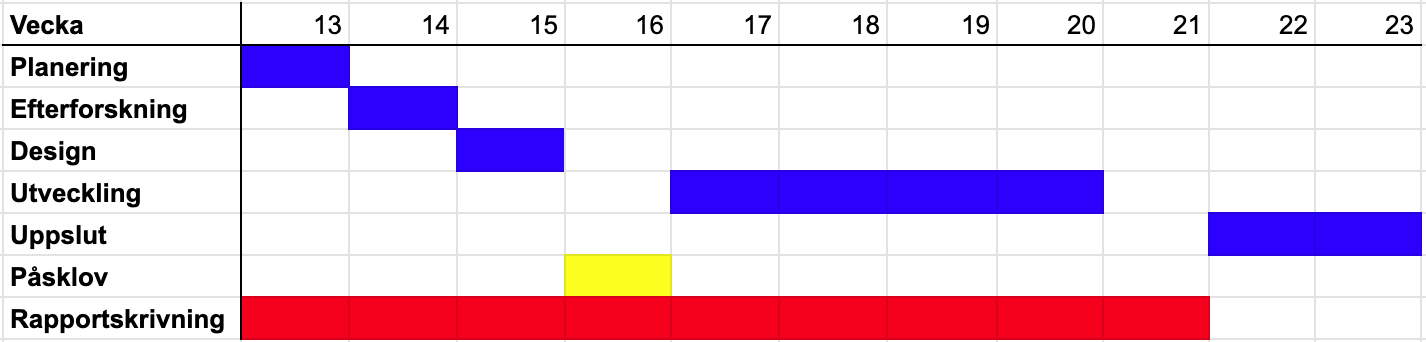
\includegraphics[width = \textwidth]{TidsplanGantt.png}
%    \caption{Gantt-diagram för vår tidsplanering}
%    \label{fig:tidplan}
%\end{figure}

%Då kursen är på heltid så är planen att det ska läggas cirka 40 timmar per vecka per student på projektet, då inkluderas även rapportskrivandet.

%Våra milstolpar är inte fastspikade än, då vår design inte är designad.

%Men de preliminära milstolparna är att designen av vårt system ska vara färdig vecka 15, chatgränssnittet vecka 17, avtalsskaparen vecka 18 och servern vecka 19.

%\section{Hur man gör appendix}
%Appendixar kan vara bra för bilagor som enkätundersökningar, större kodavsnitt, etc. 
%
%Appendix läggs efter referenslistan, och ska börja på en ny sida. Använd \verb|\newpage| för att göra ett sidbrott där resten av nuvarande sida är tom. Skriv sen \verb|\appendix| för att markera att resten är appendix, och 
% använd sen vanliga \verb|\section{}| för varje appendix, som kommer att ``numreras'' A, B, C osv.
%
%\section{Några tips för La\TeX-användning}
%
%Ett enkelt sätt att använda/\textbf{installera} LaTeX för MacOS är TexShop (\url{http://pages.uoregon.edu/koch/texshop}).
%
%För \textbf{samarbete} när man skriver La\TeX-dokument använder somliga Overleaf (\url{https://www.overleaf.com/}, tips på liknande system är välkomna), men det funkar också att använda git och vanliga texteditorer (t.ex Emacs). I det fallet är det smart att dela upp dokumentet i flera (t.ex. ett per kapitel) som sen inkluderas med \verb|\input{kapitel}|. Ett tips är också att slå på radbrytning i texteditorn, så att konflikter vid incheckningar hanteras per kort rad istället för per jättelång rad.
%
%\textbf{Läs också i Wikibooks} (\url{http://en.wikibooks.org/wiki/LaTeX}), \textbf{missa inte} Appendix om ``Sample LaTeX documents'' (men använd alltid rapportmallen som bas).
%
%\textbf{Citat-tecken} skriver man med \verb|``foo''| (dvs två bakåtfnuttar före, och två vanliga fnuttar efter). LaTeX gör så att det blir snyggt: ``foo''.
%
%När man skriver på svenska behöver man ibland ``visa'' var ord (speciellt såna med med åäö) kan \textbf{avstavas} genom att använda \verb|\-| (liknande \textit{soft hyphen}): ämnesöversiktsintroduktion avstavas med några sådana instuckna på rätt ställen istället som ämnes\-över\-sikts\-intro\-duk\-tion
%
%\begin{verbatim}
%ämnes\-över\-sikts\-intro\-duk\-tion
%\end{verbatim}
%
%För att formattera \textbf{URLer} bättre (så att t.ex. radbrytning blir snyggare), skriv t.ex. \verb|\url{http://www.it.uu.se/research/group/concurrency}| i texten eller referensen.
%
%För att \textbf{referera} till avsnitt, figurer, tabeller etc, använd \verb|\label{markör}| för att ``sätta ett märke'' i text eller figur, och \verb|\ref{markör}| för att referera till den, t.ex.
%\begin{verbatim}
%\section{Motivation}
%\label{sec:motivation}
%\end{verbatim}
%
%följt av
%\begin{verbatim}
%Som vi nämnt i avsnitt~\ref{sec.motivation}...
%\end{verbatim}
%
%För att få referenser att inte hamna först efter ett \textbf{radbrott}, använd icke-brytande space \verb|såhär~\cite{fin-bok}|, där tilde-tecknet \verb|~| alltså gör ett obrytbart space. Detta är i princip också alltid rätt att använda före siffror, och förstås också före \verb|\ref{fig}|.
%
%Använd \emph{aldrig} dubbel-backslash \verb|\\| för att få avbrott mellan stycken. Använd alltid dubbel ny rad för detta.
%
%För att göra ett \textbf{sidbrott} där resten av sidan blir tom, använd \verb|\newpage|, inte \verb|\pagebreak|. Det senare är till för att finjustera var latex gör ett automatiskt sidbrott, inte för att avsluta en halvfull sida.
%
%\subsection{Bib\TeX-tips}
%
%För att hantera bibliografi (\textbf{referenser}) på ett smidigt sätt, använd BibTeX! (se \url{http://en.wikibooks.org/wiki/LaTeX/Bibliography_Management#BibTeX} och nedan om referenser.)
%
%För att se till att BibTeX inte gör namn, förkortningar etc till lowercase, använd \verb|{}| och skriv typ
%\begin{verbatim}
%title = {The {DSP} of {N}ewton applied to {iOS}}
%\end{verbatim}
%
%Skriv alltid månader för publikation med de inbyggda förkortningarna, typ:
%\begin{verbatim}
%month = jun
%\end{verbatim}
%istället för \verb|{jun}| eller \verb|"jun"| eller \verb|"June"| eller \verb|"Juni"|. Då kan nämligen bibliographystyle styra hur det förkortas etc.
%
%Ett verktyg för att hantera BibTeX-filer i MacOS är BibDesk (\url{http://bibdesk.sourceforge.net/}).
%
%\section{Referenser}
%\label{sec:referenser}
%
%Se också kap 8.5 i Dawson~\cite{dawson:projects-in-computing}.
%
%Det finns åtminstone tre syften med utformningen av referenserna och referenslistan.
%\begin{enumerate}
%\item Man ska hitta referensen (från texten) i referenslistan.
%\item Man ska förstå vad som refereras (vilken typ av referens det är) så att man kan värdera den.
%\item Man ska kunna hitta referensen i verkligheten.
%\end{enumerate}
%
%Använd numeriska referenser (IEEE-stil~[42]) eller nyckelordsbaserad~[Lam86], inte fotnotstil. Referenserna sorteras alfabetiskt efter författare/motsv i referenslistan. I LaTeX, använd \verb|\bibliographystyle{IEEEtranS}| eller \verb|{IEEEtranSA}| (eller liknande), se rapportmallen. \textbf{Börja} med att använda \verb|{IEEEtranSA}| som tydligare visar när viss info saknas i bibtex-entries (t.ex. år och författare).
%
%För att göra inställningar för \verb|\bibliographystyle{IEEEtranS/SA}| kan man använda ett speciellt bibtex-entry \texttt{@IEEEtranBSTCTL}, se \texttt{IEEEtran\_bst\_HOWTO.pdf} i directoryt \texttt{IEEEtran/bibtex}, avsnitt VII, eller sista biten av \texttt{IEEEexample.bib} i samma directory.
%
%Referenserna skrivs i direkt anknytning till det som föranleder referensen (t.ex. ett påstående eller resultat), före eventuellt skiljetecken, och med ett fast mellanslag till föregående ord. I La\TeX, \verb|skriv~\cite{lam86}| för att få en ``non-breaking space''. Se också rapportmallen, och sista stycket på sid 211 i Dawson~\cite{dawson:projects-in-computing}. 
%
%Det är alltså \emph{inte} en bra approach att skriva referenserna efter ett längre stycke (som vissa verkar lära sig att göra, någonstans). Det gör det oftast otydligt vad som egentligen är hämtat från, eller styrks, av referenserna. I vissa fall kan man vilka göra en kort sammanfattning av vad en författare skriver i en artikel el.dyl., men att bara lägga på en referens sist i stycket är inte tillräckligt tydligt. Det är mycket bättre och tydligare att skriva något i stil med ``Lisa Lagom beskriver\verb|~\cite{lagom-bok}| hur X beror av Y och i sin analys visar hon i detalj hur sambandet ser ut\ldots''.
%
%När man refererar till ``tjocka'' saker som böcker är det lämpligt att ange sidnr 
%(som \verb|\cite[sid 211-214]{dawson:projects-in-computing}|) som blir~\cite[sid 211-214]{dawson:projects-in-computing}, men för ``tunnare'' saker behöver man bara göra det för att speciellt peka ut om man t.ex. menar en viss del av referensen (kanske den tar upp tre olika sätt att göra X och man vill peka på det 3:e, inte de första två).
%
%För mer info om vilken info som behövs för olika typer av referenser, se avsnitt 8.5.3 i Dawson~\cite{dawson:projects-in-computing,dawson:projects-in-computing-old}. (För att referera till flera saker samtidigt (som nyss) skriver man flera BibTeX-nycklar i samma \verb|\cite|.)
%
%Använd inte direktcitat, såvida inte den exakta formuleringen är viktig.  Skriv hellre ett referat av vad någon sagt. (Se Dawson.)
%
%Om referenslistan huvudsakligen innehåller referenser till ``mer info'' av typen 
%\url{www.wordpress.org}, \url{www.w3c.org}, \url{developer.android.com}\ldots men få referenser som stöder resonemang, motivation, argument etc (jfr Workshoparna), är det antagligen ett tecken på att det finns få resonemang, motiveringar och argument som behöver stödjas. Då behöver man med största sannolikhet resonera, motivera och argumentera mera!
%
%Även om en referens har en URL till själva texten är det inte nödvändigtvis en webbreferens, utan ibland en artikel/bok el.dyl som råkar vara tllgänglig på nätet. Den ska då beskrivas som artikel/bok/el.dyl (men förstås gärna med URLen) så att man kan göra en preliminär värdering av referensen redan när man läser referenslistan.
%
%Försök hitta författare och publiceringsdatum (år, månad) även för webbreferenser, och ange när de lästes. Ett exempel är~\cite{berners-lee:cool-uris} (se \texttt{refs.bib}).
%
%
%
%\section{Formler, figurer, bilder, kod}
%\label{sec:forml-figur-bild}
%
%Formler, figurer och ekvationer måste beskrivas.  Det betyder t.ex. att varje symbol måste vara förklarad i texten.
%
%I engelsk text skriver man ``Figure 3'', inte ``figure 3'', eftersom det fungerar som ett namn på figuren (och motsvarande för Table, Section osv).
%
%Alla figurer och bilder som inte är era egna måste ha referenser till källan.
%
%Rapportmallen är inställd så att figurer presenteras med en linje över, en under, och en mellan figurtexten och själva bilden. För andra presentationer, se macrot \verb|\floatstyle| (googla) -- exempelvis ger \verb|\floatstyle{boxed}| istället en ram runt figuren.
%
%Om ni inkluderar kodsnuttar, se till att de är relevanta och kommenterade, så att man förstår.  Alternativt, för korta snuttar: ge motsvarande förklaring i texten.
%Använd vettigt latex-bibliotek för kod, t.ex. \texttt{listings}.
%
%\section{Språk och grammatik}
%\label{sec:sprak-och-grammatik}
%
%\begin{itemize}
%\item    Det är OK att skriva ``Vi''!
%
%\item    \textbf{Inte alla läsare är män}.  Skriv därför inte ``han'', ``hans'', ``denne'' etc.  Använd könsneutrala pronomen eller ord som ``vederbörande'', ``användaren'' etc.
%
%\item    \textbf{Undvik talspråk} ``så'', ``två stycken saker'', ``ifrån'', ``av'', ``vart'', ``kommer göra/vara'' (istället för ``kommer att göra/vara'', \ldots \textbf{Kolla på Wikipedia-sidan} ``Vanliga språkfel''~\cite{wp:sprakfel} (länk i vänsterkanten i SP).
%
%\item    Undvik värderande uttryck som enkelt, uppenbart.
%
%\item Undvik att sluta meningar med en preposition (t.ex. \emph{med} eller \emph{with}).
%
%\item På engelska, undvik det informella \emph{you} som översättning av ``man'' -- undvik också \emph{one} som kan upplevas som alltför formellt (drottningen uttrycker sig så). Skriv ut vem som menas, t.ex. ``the user'' el.dyl.
%
%\item    Semikolon är \textbf{inte} en variant av kolon eller komma; semikolon kan endast användas där ni normalt sett skulle använt punkt, men vill fortsätta på samma mening. För att undvika problem, undvik semikolon helt.
%
%\item    Skriv inte meningar som börjar med ``Detta på grund av'' eller ``Detta eftersom\ldots' -- det blir ofta inte fullständiga meningar och det är ofta inte klart vad ``detta'' syftar på.
%
%\item    Använd inte framtid (futurum); skriv rapporten i nu- eller dåtid och var konsekventa (Vi gör\ldots eller Vi har gjort\ldots, inte Vi kommer att göra\ldots)
%
%\item    \textbf{Förklara begrepp innan ni använder dem}, hänvisa inte \emph{bara} läsaren till ett senare avsnitt (men ni kan naturligtvis också hänvisa till mer detaljerade förklaringar som kommer senare i texten).  Första gången ett begrepp nämns måste alltså åtminstone en kort förklaring finnas.
%
%\item    När ni introducerar nya koncept (sådant ni inte har diskuterat tidigare), gör inte det ``i förbifarten'', utan se till att ni \textbf{förklarar ordentligt}.  Alltså: ``Vi använder X (ett häftigt nytt programmeringsspråk) för att göra Y'' fungerar inte.  Beskriv först konceptet ni använder, och använd det sedan.  Typ ``X är ett viktigt nytt programmeringsspråk.  Vi använder X för att göra Y.''
%
%\item    \textbf{Var konsekventa} med hur ni skriver förkortningar och begrepp (c++ eller C++, android och Android t.ex.) Tumregel: namn skrivs med inledande stor bokstav (Android, inte android), förkortningar med stora bokstäver (XML, inte Xml).
%
%\item    Använd inte olika synonymer för det ni har utvecklat (tjänsten/projektet/systemet), utan bestäm er för vad ni kallar det ni har gjort.
%
%\item    Det kan vara bra att kursivera nya begrepp första gången de används, men normalt bör man inte kursivera \emph{alla} förekomster.
%
%\item    Efter uttryck som ``för det första\ldots'', ``one alternative is\ldots'' måste följa ``för det andra\ldots'' ``another alternative'' (inte ``slutligen'', ``dels'', ``another \underline{option}'' eller något annat).  Tänk också på ``firstly \ldots secondly'' resp. ``first \ldots second'', inte ``first \ldots secondly'' eller något annat.
%
%\item    Var försiktig med uttryck som ``this approach'', ``detta system'', etc. och kontrollera att det är uppenbart vad detta/this refererar till. Be någon icke-gruppmedlem läsa och kolla!
%
%\item    De av er som skriver på engelska: ni MÅSTE använda korrekta verbformer beroende på om subjektet är en eller flera saker (``it has'' men ``they have'').
%\end{itemize}

\end{document}
